\documentclass[twoside]{book}

% Packages required by doxygen
\usepackage{fixltx2e}
\usepackage{calc}
\usepackage{doxygen}
\usepackage[export]{adjustbox} % also loads graphicx
\usepackage{graphicx}
\usepackage[utf8]{inputenc}
\usepackage{makeidx}
\usepackage{multicol}
\usepackage{multirow}
\PassOptionsToPackage{warn}{textcomp}
\usepackage{textcomp}
\usepackage[nointegrals]{wasysym}
\usepackage[table]{xcolor}

% Font selection
\usepackage[T1]{fontenc}
\usepackage[scaled=.90]{helvet}
\usepackage{courier}
\usepackage{amssymb}
\usepackage{sectsty}
\renewcommand{\familydefault}{\sfdefault}
\allsectionsfont{%
  \fontseries{bc}\selectfont%
  \color{darkgray}%
}
\renewcommand{\DoxyLabelFont}{%
  \fontseries{bc}\selectfont%
  \color{darkgray}%
}
\newcommand{\+}{\discretionary{\mbox{\scriptsize$\hookleftarrow$}}{}{}}

% Page & text layout
\usepackage{geometry}
\geometry{%
  a4paper,%
  top=2.5cm,%
  bottom=2.5cm,%
  left=2.5cm,%
  right=2.5cm%
}
\tolerance=750
\hfuzz=15pt
\hbadness=750
\setlength{\emergencystretch}{15pt}
\setlength{\parindent}{0cm}
\setlength{\parskip}{3ex plus 2ex minus 2ex}
\makeatletter
\renewcommand{\paragraph}{%
  \@startsection{paragraph}{4}{0ex}{-1.0ex}{1.0ex}{%
    \normalfont\normalsize\bfseries\SS@parafont%
  }%
}
\renewcommand{\subparagraph}{%
  \@startsection{subparagraph}{5}{0ex}{-1.0ex}{1.0ex}{%
    \normalfont\normalsize\bfseries\SS@subparafont%
  }%
}
\makeatother

% Headers & footers
\usepackage{fancyhdr}
\pagestyle{fancyplain}
\fancyhead[LE]{\fancyplain{}{\bfseries\thepage}}
\fancyhead[CE]{\fancyplain{}{}}
\fancyhead[RE]{\fancyplain{}{\bfseries\leftmark}}
\fancyhead[LO]{\fancyplain{}{\bfseries\rightmark}}
\fancyhead[CO]{\fancyplain{}{}}
\fancyhead[RO]{\fancyplain{}{\bfseries\thepage}}
\fancyfoot[LE]{\fancyplain{}{}}
\fancyfoot[CE]{\fancyplain{}{}}
\fancyfoot[RE]{\fancyplain{}{\bfseries\scriptsize Generated by Doxygen }}
\fancyfoot[LO]{\fancyplain{}{\bfseries\scriptsize Generated by Doxygen }}
\fancyfoot[CO]{\fancyplain{}{}}
\fancyfoot[RO]{\fancyplain{}{}}
\renewcommand{\footrulewidth}{0.4pt}
\renewcommand{\chaptermark}[1]{%
  \markboth{#1}{}%
}
\renewcommand{\sectionmark}[1]{%
  \markright{\thesection\ #1}%
}

% Indices & bibliography
\usepackage{natbib}
\usepackage[titles]{tocloft}
\setcounter{tocdepth}{3}
\setcounter{secnumdepth}{5}
\makeindex

% Hyperlinks (required, but should be loaded last)
\usepackage{ifpdf}
\ifpdf
  \usepackage[pdftex,pagebackref=true]{hyperref}
\else
  \usepackage[ps2pdf,pagebackref=true]{hyperref}
\fi
\hypersetup{%
  colorlinks=true,%
  linkcolor=blue,%
  citecolor=blue,%
  unicode%
}

% Custom commands
\newcommand{\clearemptydoublepage}{%
  \newpage{\pagestyle{empty}\cleardoublepage}%
}

\usepackage{caption}
\captionsetup{labelsep=space,justification=centering,font={bf},singlelinecheck=off,skip=4pt,position=top}

%===== C O N T E N T S =====

\begin{document}

% Titlepage & ToC
\hypersetup{pageanchor=false,
             bookmarksnumbered=true,
             pdfencoding=unicode
            }
\pagenumbering{alph}
\begin{titlepage}
\vspace*{7cm}
\begin{center}%
{\Large Babel\+\_\+2019 \\[1ex]\large Alpha 1.\+0 }\\
\vspace*{1cm}
{\large Generated by Doxygen 1.8.13}\\
\end{center}
\end{titlepage}
\clearemptydoublepage
\pagenumbering{roman}
\tableofcontents
\clearemptydoublepage
\pagenumbering{arabic}
\hypersetup{pageanchor=true}

%--- Begin generated contents ---
\chapter{Hierarchical Index}
\section{Class Hierarchy}
This inheritance list is sorted roughly, but not completely, alphabetically\+:\begin{DoxyCompactList}
\item \contentsline{section}{cli\+:\+:Client}{\pageref{classcli_1_1_client}}{}
\item \contentsline{section}{Client}{\pageref{class_client}}{}
\item \contentsline{section}{Client\+Actions}{\pageref{class_client_actions}}{}
\item \contentsline{section}{Client\+Database}{\pageref{class_client_database}}{}
\item \contentsline{section}{db\+:\+:Data}{\pageref{classdb_1_1_data}}{}
\begin{DoxyCompactList}
\item \contentsline{section}{db\+:\+:Client\+Database}{\pageref{classdb_1_1_client_database}}{}
\end{DoxyCompactList}
\item \contentsline{section}{Data}{\pageref{class_data}}{}
\item \contentsline{section}{db\+:\+:Database}{\pageref{classdb_1_1_database}}{}
\item \contentsline{section}{Database}{\pageref{class_database}}{}
\item \contentsline{section}{Encoder\+System}{\pageref{class_encoder_system}}{}
\item \contentsline{section}{Client\+Actions\+:\+:info\+\_\+s}{\pageref{struct_client_actions_1_1info__s}}{}
\item \contentsline{section}{utils\+:\+:Packet}{\pageref{classutils_1_1_packet}}{}
\item \contentsline{section}{pa\+Test\+Data}{\pageref{structpa_test_data}}{}
\item \contentsline{section}{Port\+Audio}{\pageref{class_port_audio}}{}
\item \contentsline{section}{cli\+:\+:props\+\_\+s}{\pageref{structcli_1_1props__s}}{}
\item \contentsline{section}{qt\+\_\+meta\+\_\+stringdata\+\_\+main\+Window\+\_\+t}{\pageref{structqt__meta__stringdata__main_window__t}}{}
\item Q\+Widget\begin{DoxyCompactList}
\item \contentsline{section}{main\+Window}{\pageref{classmain_window}}{}
\end{DoxyCompactList}
\item \contentsline{section}{Server}{\pageref{class_server}}{}
\item \contentsline{section}{Server\+Actions}{\pageref{class_server_actions}}{}
\begin{DoxyCompactList}
\item \contentsline{section}{ns\+:\+:Server}{\pageref{classns_1_1_server}}{}
\end{DoxyCompactList}
\item \contentsline{section}{Server\+Client}{\pageref{class_server_client}}{}
\item \contentsline{section}{Socket}{\pageref{class_socket}}{}
\item \contentsline{section}{T\+C\+P\+Socket}{\pageref{class_t_c_p_socket}}{}
\item \contentsline{section}{U\+D\+P\+Socket}{\pageref{class_u_d_p_socket}}{}
\item \contentsline{section}{Ui\+\_\+\+Main\+Window}{\pageref{class_ui___main_window}}{}
\begin{DoxyCompactList}
\item \contentsline{section}{Ui\+:\+:Main\+Window}{\pageref{class_ui_1_1_main_window}}{}
\end{DoxyCompactList}
\end{DoxyCompactList}

\chapter{Class Index}
\section{Class List}
Here are the classes, structs, unions and interfaces with brief descriptions\+:\begin{DoxyCompactList}
\item\contentsline{section}{\hyperlink{classcli_1_1_client}{cli\+::\+Client} }{\pageref{classcli_1_1_client}}{}
\item\contentsline{section}{\hyperlink{class_client}{Client} \\*Class representing the \hyperlink{class_client}{Client} }{\pageref{class_client}}{}
\item\contentsline{section}{\hyperlink{class_client_actions}{Client\+Actions} \\*Class representing the \hyperlink{class_client_actions}{Client\+Actions} }{\pageref{class_client_actions}}{}
\item\contentsline{section}{\hyperlink{classdb_1_1_client_database}{db\+::\+Client\+Database} }{\pageref{classdb_1_1_client_database}}{}
\item\contentsline{section}{\hyperlink{class_client_database}{Client\+Database} \\*Class representing the \hyperlink{class_client_database}{Client\+Database} }{\pageref{class_client_database}}{}
\item\contentsline{section}{\hyperlink{classdb_1_1_data}{db\+::\+Data} }{\pageref{classdb_1_1_data}}{}
\item\contentsline{section}{\hyperlink{class_data}{Data} \\*Class representing the \hyperlink{class_data}{Data} }{\pageref{class_data}}{}
\item\contentsline{section}{\hyperlink{classdb_1_1_database}{db\+::\+Database} }{\pageref{classdb_1_1_database}}{}
\item\contentsline{section}{\hyperlink{class_database}{Database} \\*Class representing the \hyperlink{class_database}{Database} }{\pageref{class_database}}{}
\item\contentsline{section}{\hyperlink{class_encoder_system}{Encoder\+System} }{\pageref{class_encoder_system}}{}
\item\contentsline{section}{\hyperlink{struct_client_actions_1_1info__s}{Client\+Actions\+::info\+\_\+s} }{\pageref{struct_client_actions_1_1info__s}}{}
\item\contentsline{section}{\hyperlink{classmain_window}{main\+Window} }{\pageref{classmain_window}}{}
\item\contentsline{section}{\hyperlink{class_ui_1_1_main_window}{Ui\+::\+Main\+Window} }{\pageref{class_ui_1_1_main_window}}{}
\item\contentsline{section}{\hyperlink{classutils_1_1_packet}{utils\+::\+Packet} }{\pageref{classutils_1_1_packet}}{}
\item\contentsline{section}{\hyperlink{structpa_test_data}{pa\+Test\+Data} }{\pageref{structpa_test_data}}{}
\item\contentsline{section}{\hyperlink{class_port_audio}{Port\+Audio} }{\pageref{class_port_audio}}{}
\item\contentsline{section}{\hyperlink{structcli_1_1props__s}{cli\+::props\+\_\+s} }{\pageref{structcli_1_1props__s}}{}
\item\contentsline{section}{\hyperlink{structqt__meta__stringdata__main_window__t}{qt\+\_\+meta\+\_\+stringdata\+\_\+main\+Window\+\_\+t} }{\pageref{structqt__meta__stringdata__main_window__t}}{}
\item\contentsline{section}{\hyperlink{class_server}{Server} \\*Class representing the \hyperlink{class_server}{Server} }{\pageref{class_server}}{}
\item\contentsline{section}{\hyperlink{classns_1_1_server}{ns\+::\+Server} }{\pageref{classns_1_1_server}}{}
\item\contentsline{section}{\hyperlink{class_server_actions}{Server\+Actions} \\*Class representing the \hyperlink{class_server_actions}{Server\+Actions} }{\pageref{class_server_actions}}{}
\item\contentsline{section}{\hyperlink{class_server_client}{Server\+Client} \\*Class representing the \hyperlink{class_server_client}{Server\+Client} }{\pageref{class_server_client}}{}
\item\contentsline{section}{\hyperlink{class_socket}{Socket} \\*Class representing the \hyperlink{class_socket}{Socket} }{\pageref{class_socket}}{}
\item\contentsline{section}{\hyperlink{class_t_c_p_socket}{T\+C\+P\+Socket} \\*Class representing the \hyperlink{class_t_c_p_socket}{T\+C\+P\+Socket} }{\pageref{class_t_c_p_socket}}{}
\item\contentsline{section}{\hyperlink{class_u_d_p_socket}{U\+D\+P\+Socket} \\*Class representing the \hyperlink{class_u_d_p_socket}{U\+D\+P\+Socket} }{\pageref{class_u_d_p_socket}}{}
\item\contentsline{section}{\hyperlink{class_ui___main_window}{Ui\+\_\+\+Main\+Window} }{\pageref{class_ui___main_window}}{}
\end{DoxyCompactList}

\chapter{Class Documentation}
\hypertarget{classcli_1_1_client}{}\section{cli\+:\+:Client Class Reference}
\label{classcli_1_1_client}\index{cli\+::\+Client@{cli\+::\+Client}}
\subsection*{Public Member Functions}
\begin{DoxyCompactItemize}
\item 
\mbox{\Hypertarget{classcli_1_1_client_a135ecc70f5ac2e08199c0bcd35ed7ea6}\label{classcli_1_1_client_a135ecc70f5ac2e08199c0bcd35ed7ea6}} 
bool {\bfseries auth} ()
\item 
\mbox{\Hypertarget{classcli_1_1_client_af03de9c208ae4568fd41e3fe0dab8fc5}\label{classcli_1_1_client_af03de9c208ae4568fd41e3fe0dab8fc5}} 
bool {\bfseries connection} (const std\+::string \&ip, const std\+::string \&port, const std\+::string \&name)
\item 
\mbox{\Hypertarget{classcli_1_1_client_a6ca368944dd2a787e7c244d34c0b99ce}\label{classcli_1_1_client_a6ca368944dd2a787e7c244d34c0b99ce}} 
bool {\bfseries connect\+To\+Server} (const std\+::string \&ip, unsigned short port)
\item 
\mbox{\Hypertarget{classcli_1_1_client_ae0bc335d720265d4d6e8a72cf7a2a9aa}\label{classcli_1_1_client_ae0bc335d720265d4d6e8a72cf7a2a9aa}} 
void {\bfseries run} ()
\item 
\mbox{\Hypertarget{classcli_1_1_client_aea7f1e7aef5acaaecd40476e63063f05}\label{classcli_1_1_client_aea7f1e7aef5acaaecd40476e63063f05}} 
void {\bfseries init\+Streaming} ()
\item 
\mbox{\Hypertarget{classcli_1_1_client_a14f480bd5001f94e73268462274947b7}\label{classcli_1_1_client_a14f480bd5001f94e73268462274947b7}} 
void {\bfseries send\+Message} (const int clientfd, const std\+::string \&msg)
\end{DoxyCompactItemize}
\subsection*{Static Public Member Functions}
\begin{DoxyCompactItemize}
\item 
\mbox{\Hypertarget{classcli_1_1_client_aefa4c51c339bb1e1c1e9854e67ae1367}\label{classcli_1_1_client_aefa4c51c339bb1e1c1e9854e67ae1367}} 
static void {\bfseries open\+Stream} ()
\item 
\mbox{\Hypertarget{classcli_1_1_client_ad2cdcf3ed4ef4b588cc4b79cefb857e6}\label{classcli_1_1_client_ad2cdcf3ed4ef4b588cc4b79cefb857e6}} 
static void {\bfseries send\+Stream} ()
\item 
\mbox{\Hypertarget{classcli_1_1_client_a5646c53b99cbbde85ba917e81d53dbae}\label{classcli_1_1_client_a5646c53b99cbbde85ba917e81d53dbae}} 
static void {\bfseries ask\+For\+Call} (\hyperlink{class_u_d_p_socket}{U\+D\+P\+Socket})
\item 
\mbox{\Hypertarget{classcli_1_1_client_a9bd449f1ba2df2727e6cc4a1b1db1f78}\label{classcli_1_1_client_a9bd449f1ba2df2727e6cc4a1b1db1f78}} 
static void {\bfseries send\+Infos} (\hyperlink{class_t_c_p_socket}{T\+C\+P\+Socket} $\ast$, props\+\_\+p)
\item 
\mbox{\Hypertarget{classcli_1_1_client_ab3bf0efdc0b25735c0f2c1df93ef2f29}\label{classcli_1_1_client_ab3bf0efdc0b25735c0f2c1df93ef2f29}} 
static void {\bfseries new\+Connection} (\hyperlink{class_t_c_p_socket}{T\+C\+P\+Socket} $\ast$, props\+\_\+p)
\end{DoxyCompactItemize}


The documentation for this class was generated from the following files\+:\begin{DoxyCompactItemize}
\item 
network/include/Client.\+hpp\item 
network/client/Client.\+cpp\end{DoxyCompactItemize}

\hypertarget{class_client}{}\section{Client Class Reference}
\label{class_client}\index{Client@{Client}}


Class representing the \hyperlink{class_client}{Client}.  




{\ttfamily \#include $<$Client.\+hpp$>$}



\subsection{Detailed Description}
Class representing the \hyperlink{class_client}{Client}. 

This class handle the \hyperlink{class_client}{Client} 

The documentation for this class was generated from the following file\+:\begin{DoxyCompactItemize}
\item 
network/include/Client.\+hpp\end{DoxyCompactItemize}

\hypertarget{class_client_actions}{}\section{Client\+Actions Class Reference}
\label{class_client_actions}\index{Client\+Actions@{Client\+Actions}}


Class representing the \hyperlink{class_client_actions}{Client\+Actions}.  




{\ttfamily \#include $<$Client\+Actions.\+hpp$>$}

\subsection*{Classes}
\begin{DoxyCompactItemize}
\item 
struct \hyperlink{struct_client_actions_1_1info__s}{info\+\_\+s}
\end{DoxyCompactItemize}
\subsection*{Public Member Functions}
\begin{DoxyCompactItemize}
\item 
\mbox{\Hypertarget{class_client_actions_a81f8aa1801522eb7ee650cd1b4a1fb73}\label{class_client_actions_a81f8aa1801522eb7ee650cd1b4a1fb73}} 
bool {\bfseries send\+Infos} (const \hyperlink{struct_client_actions_1_1info__s}{info\+\_\+s} \&)
\end{DoxyCompactItemize}


\subsection{Detailed Description}
Class representing the \hyperlink{class_client_actions}{Client\+Actions}. 

This class handle the \hyperlink{class_client_actions}{Client\+Actions} 

The documentation for this class was generated from the following file\+:\begin{DoxyCompactItemize}
\item 
network/include/Client\+Actions.\+hpp\end{DoxyCompactItemize}

\hypertarget{classdb_1_1_client_database}{}\section{db\+:\+:Client\+Database Class Reference}
\label{classdb_1_1_client_database}\index{db\+::\+Client\+Database@{db\+::\+Client\+Database}}
Inheritance diagram for db\+:\+:Client\+Database\+:\begin{figure}[H]
\begin{center}
\leavevmode
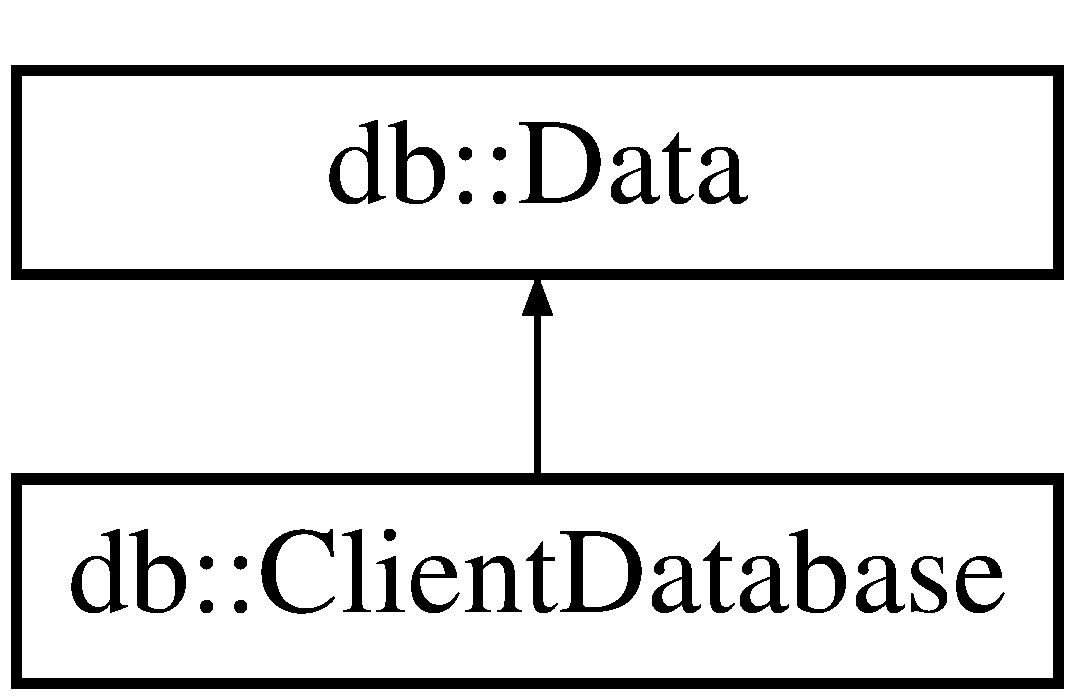
\includegraphics[height=2.000000cm]{classdb_1_1_client_database}
\end{center}
\end{figure}
\subsection*{Public Member Functions}
\begin{DoxyCompactItemize}
\item 
\hyperlink{classdb_1_1_client_database_abdb82edc1ea955df62b5514e40397622}{Client\+Database} ()
\begin{DoxyCompactList}\small\item\em ? \end{DoxyCompactList}\item 
\hyperlink{classdb_1_1_client_database_ad35c5aec453015e7785079f70fd20bb4}{Client\+Database} (const std\+::string \&)
\begin{DoxyCompactList}\small\item\em ? \end{DoxyCompactList}\item 
\hyperlink{classdb_1_1_client_database_a59973465f454ada5665d274c7565a4ec}{Client\+Database} (const std\+::string \&, time\+\_\+t \&)
\begin{DoxyCompactList}\small\item\em ? \end{DoxyCompactList}\item 
\hyperlink{classdb_1_1_client_database_af0249c4d0a723a6a39684895f226e40d}{$\sim$\+Client\+Database} ()
\begin{DoxyCompactList}\small\item\em ? \end{DoxyCompactList}\item 
void \hyperlink{classdb_1_1_client_database_aac37cb276baf5a7e63d87a7ceb2f70ca}{set\+I\+P\+Addr} (const IP \&) noexcept
\begin{DoxyCompactList}\small\item\em ? \end{DoxyCompactList}\item 
IP \hyperlink{classdb_1_1_client_database_a7300e226455d344798c75c3232b1218a}{get\+I\+P\+Addr} () const
\begin{DoxyCompactList}\small\item\em ? \end{DoxyCompactList}\item 
std\+::string \hyperlink{classdb_1_1_client_database_ad342a032236484edb6df718d7ee746b1}{get\+Insertion\+Query} () const noexcept
\begin{DoxyCompactList}\small\item\em ? \end{DoxyCompactList}\item 
\mbox{\Hypertarget{classdb_1_1_client_database_ab40b26d2ebc7b5f76c38fafaf59c8fb2}\label{classdb_1_1_client_database_ab40b26d2ebc7b5f76c38fafaf59c8fb2}} 
std\+::vector$<$ std\+::string $>$ {\bfseries get\+Attributes} () const noexcept
\item 
std\+::string \hyperlink{classdb_1_1_client_database_a930ad117ea6c1f1306f44db8716ab26a}{get\+Formatted\+Attributes} () const noexcept
\begin{DoxyCompactList}\small\item\em ? \end{DoxyCompactList}\item 
std\+::string \hyperlink{classdb_1_1_client_database_a70e9abb4361ecc6a0ea168a63743e093}{get\+Formatted\+Values} () const noexcept
\begin{DoxyCompactList}\small\item\em ? \end{DoxyCompactList}\end{DoxyCompactItemize}
\subsection*{Additional Inherited Members}


\subsection{Constructor \& Destructor Documentation}
\mbox{\Hypertarget{classdb_1_1_client_database_abdb82edc1ea955df62b5514e40397622}\label{classdb_1_1_client_database_abdb82edc1ea955df62b5514e40397622}} 
\index{db\+::\+Client\+Database@{db\+::\+Client\+Database}!Client\+Database@{Client\+Database}}
\index{Client\+Database@{Client\+Database}!db\+::\+Client\+Database@{db\+::\+Client\+Database}}
\subsubsection{\texorpdfstring{Client\+Database()}{ClientDatabase()}\hspace{0.1cm}{\footnotesize\ttfamily [1/3]}}
{\footnotesize\ttfamily Client\+Database\+::\+Client\+Database (\begin{DoxyParamCaption}{ }\end{DoxyParamCaption})}



? 


\begin{DoxyParams}{Parameters}
{\em void} & \\
\hline
\end{DoxyParams}
\mbox{\Hypertarget{classdb_1_1_client_database_ad35c5aec453015e7785079f70fd20bb4}\label{classdb_1_1_client_database_ad35c5aec453015e7785079f70fd20bb4}} 
\index{db\+::\+Client\+Database@{db\+::\+Client\+Database}!Client\+Database@{Client\+Database}}
\index{Client\+Database@{Client\+Database}!db\+::\+Client\+Database@{db\+::\+Client\+Database}}
\subsubsection{\texorpdfstring{Client\+Database()}{ClientDatabase()}\hspace{0.1cm}{\footnotesize\ttfamily [2/3]}}
{\footnotesize\ttfamily Client\+Database\+::\+Client\+Database (\begin{DoxyParamCaption}\item[{const std\+::string \&}]{name }\end{DoxyParamCaption})}



? 


\begin{DoxyParams}{Parameters}
{\em const} & std\+::string \&name \\
\hline
\end{DoxyParams}
\mbox{\Hypertarget{classdb_1_1_client_database_a59973465f454ada5665d274c7565a4ec}\label{classdb_1_1_client_database_a59973465f454ada5665d274c7565a4ec}} 
\index{db\+::\+Client\+Database@{db\+::\+Client\+Database}!Client\+Database@{Client\+Database}}
\index{Client\+Database@{Client\+Database}!db\+::\+Client\+Database@{db\+::\+Client\+Database}}
\subsubsection{\texorpdfstring{Client\+Database()}{ClientDatabase()}\hspace{0.1cm}{\footnotesize\ttfamily [3/3]}}
{\footnotesize\ttfamily Client\+Database\+::\+Client\+Database (\begin{DoxyParamCaption}\item[{const std\+::string \&}]{name,  }\item[{time\+\_\+t \&}]{last\+Modified\+Date }\end{DoxyParamCaption})}



? 


\begin{DoxyParams}{Parameters}
{\em const} & std\+::string \&name, time\+\_\+t \&last\+Modified\+Date \\
\hline
\end{DoxyParams}
\mbox{\Hypertarget{classdb_1_1_client_database_af0249c4d0a723a6a39684895f226e40d}\label{classdb_1_1_client_database_af0249c4d0a723a6a39684895f226e40d}} 
\index{db\+::\+Client\+Database@{db\+::\+Client\+Database}!````~Client\+Database@{$\sim$\+Client\+Database}}
\index{````~Client\+Database@{$\sim$\+Client\+Database}!db\+::\+Client\+Database@{db\+::\+Client\+Database}}
\subsubsection{\texorpdfstring{$\sim$\+Client\+Database()}{~ClientDatabase()}}
{\footnotesize\ttfamily Client\+Database\+::$\sim$\+Client\+Database (\begin{DoxyParamCaption}{ }\end{DoxyParamCaption})}



? 


\begin{DoxyParams}{Parameters}
{\em void} & \\
\hline
\end{DoxyParams}


\subsection{Member Function Documentation}
\mbox{\Hypertarget{classdb_1_1_client_database_a930ad117ea6c1f1306f44db8716ab26a}\label{classdb_1_1_client_database_a930ad117ea6c1f1306f44db8716ab26a}} 
\index{db\+::\+Client\+Database@{db\+::\+Client\+Database}!get\+Formatted\+Attributes@{get\+Formatted\+Attributes}}
\index{get\+Formatted\+Attributes@{get\+Formatted\+Attributes}!db\+::\+Client\+Database@{db\+::\+Client\+Database}}
\subsubsection{\texorpdfstring{get\+Formatted\+Attributes()}{getFormattedAttributes()}}
{\footnotesize\ttfamily std\+::string Client\+Database\+::get\+Formatted\+Attributes (\begin{DoxyParamCaption}{ }\end{DoxyParamCaption}) const\hspace{0.3cm}{\ttfamily [virtual]}, {\ttfamily [noexcept]}}



? 


\begin{DoxyParams}{Parameters}
{\em void} & \\
\hline
\end{DoxyParams}


Implements \hyperlink{classdb_1_1_data}{db\+::\+Data}.

\mbox{\Hypertarget{classdb_1_1_client_database_a70e9abb4361ecc6a0ea168a63743e093}\label{classdb_1_1_client_database_a70e9abb4361ecc6a0ea168a63743e093}} 
\index{db\+::\+Client\+Database@{db\+::\+Client\+Database}!get\+Formatted\+Values@{get\+Formatted\+Values}}
\index{get\+Formatted\+Values@{get\+Formatted\+Values}!db\+::\+Client\+Database@{db\+::\+Client\+Database}}
\subsubsection{\texorpdfstring{get\+Formatted\+Values()}{getFormattedValues()}}
{\footnotesize\ttfamily std\+::string Client\+Database\+::get\+Formatted\+Values (\begin{DoxyParamCaption}{ }\end{DoxyParamCaption}) const\hspace{0.3cm}{\ttfamily [noexcept]}}



? 


\begin{DoxyParams}{Parameters}
{\em void} & \\
\hline
\end{DoxyParams}
\mbox{\Hypertarget{classdb_1_1_client_database_ad342a032236484edb6df718d7ee746b1}\label{classdb_1_1_client_database_ad342a032236484edb6df718d7ee746b1}} 
\index{db\+::\+Client\+Database@{db\+::\+Client\+Database}!get\+Insertion\+Query@{get\+Insertion\+Query}}
\index{get\+Insertion\+Query@{get\+Insertion\+Query}!db\+::\+Client\+Database@{db\+::\+Client\+Database}}
\subsubsection{\texorpdfstring{get\+Insertion\+Query()}{getInsertionQuery()}}
{\footnotesize\ttfamily std\+::string Client\+Database\+::get\+Insertion\+Query (\begin{DoxyParamCaption}{ }\end{DoxyParamCaption}) const\hspace{0.3cm}{\ttfamily [virtual]}, {\ttfamily [noexcept]}}



? 


\begin{DoxyParams}{Parameters}
{\em void} & \\
\hline
\end{DoxyParams}


Implements \hyperlink{classdb_1_1_data}{db\+::\+Data}.

\mbox{\Hypertarget{classdb_1_1_client_database_a7300e226455d344798c75c3232b1218a}\label{classdb_1_1_client_database_a7300e226455d344798c75c3232b1218a}} 
\index{db\+::\+Client\+Database@{db\+::\+Client\+Database}!get\+I\+P\+Addr@{get\+I\+P\+Addr}}
\index{get\+I\+P\+Addr@{get\+I\+P\+Addr}!db\+::\+Client\+Database@{db\+::\+Client\+Database}}
\subsubsection{\texorpdfstring{get\+I\+P\+Addr()}{getIPAddr()}}
{\footnotesize\ttfamily db\+::\+IP Client\+Database\+::get\+I\+P\+Addr (\begin{DoxyParamCaption}{ }\end{DoxyParamCaption}) const}



? 


\begin{DoxyParams}{Parameters}
{\em void} & \\
\hline
\end{DoxyParams}
\mbox{\Hypertarget{classdb_1_1_client_database_aac37cb276baf5a7e63d87a7ceb2f70ca}\label{classdb_1_1_client_database_aac37cb276baf5a7e63d87a7ceb2f70ca}} 
\index{db\+::\+Client\+Database@{db\+::\+Client\+Database}!set\+I\+P\+Addr@{set\+I\+P\+Addr}}
\index{set\+I\+P\+Addr@{set\+I\+P\+Addr}!db\+::\+Client\+Database@{db\+::\+Client\+Database}}
\subsubsection{\texorpdfstring{set\+I\+P\+Addr()}{setIPAddr()}}
{\footnotesize\ttfamily void Client\+Database\+::set\+I\+P\+Addr (\begin{DoxyParamCaption}\item[{const IP \&}]{ip\+Addr }\end{DoxyParamCaption})\hspace{0.3cm}{\ttfamily [noexcept]}}



? 


\begin{DoxyParams}{Parameters}
{\em const} & IP \&ip\+Addr \\
\hline
\end{DoxyParams}


The documentation for this class was generated from the following files\+:\begin{DoxyCompactItemize}
\item 
database/include/Client\+Database.\+hpp\item 
database/srcs/Client\+Database.\+cpp\end{DoxyCompactItemize}

\hypertarget{class_client_database}{}\section{Client\+Database Class Reference}
\label{class_client_database}\index{Client\+Database@{Client\+Database}}


Class representing the \hyperlink{class_client_database}{Client\+Database}.  




{\ttfamily \#include $<$Client\+Database.\+hpp$>$}



\subsection{Detailed Description}
Class representing the \hyperlink{class_client_database}{Client\+Database}. 

This class handle the \hyperlink{class_client_database}{Client\+Database} 

The documentation for this class was generated from the following file\+:\begin{DoxyCompactItemize}
\item 
database/include/Client\+Database.\+hpp\end{DoxyCompactItemize}

\hypertarget{classdb_1_1_data}{}\section{db\+:\+:Data Class Reference}
\label{classdb_1_1_data}\index{db\+::\+Data@{db\+::\+Data}}
Inheritance diagram for db\+:\+:Data\+:\begin{figure}[H]
\begin{center}
\leavevmode
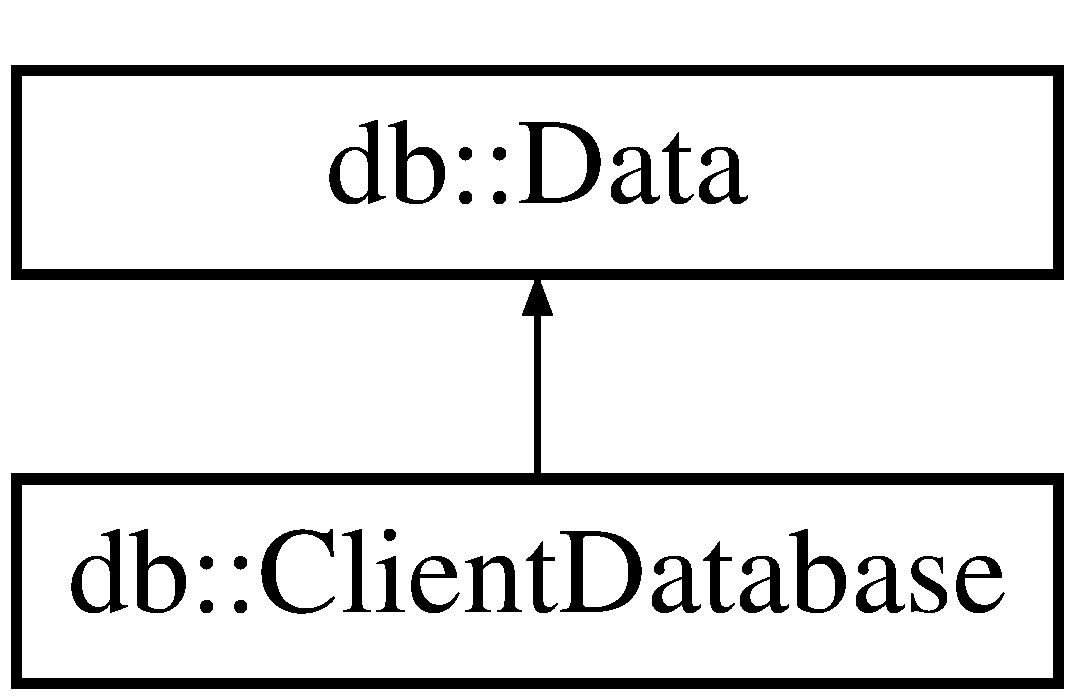
\includegraphics[height=2.000000cm]{classdb_1_1_data}
\end{center}
\end{figure}
\subsection*{Public Types}
\begin{DoxyCompactItemize}
\item 
\mbox{\Hypertarget{classdb_1_1_data_ae56789b59e6660661b4a4158d65702bb}\label{classdb_1_1_data_ae56789b59e6660661b4a4158d65702bb}} 
typedef unsigned int {\bfseries ID}
\end{DoxyCompactItemize}
\subsection*{Public Member Functions}
\begin{DoxyCompactItemize}
\item 
\mbox{\Hypertarget{classdb_1_1_data_aed9c8c04f9a4d0faff36bf7880010686}\label{classdb_1_1_data_aed9c8c04f9a4d0faff36bf7880010686}} 
{\bfseries Data} (const std\+::string \&)
\item 
\mbox{\Hypertarget{classdb_1_1_data_a79e2dc2dbadf4e565f0682a4491724e1}\label{classdb_1_1_data_a79e2dc2dbadf4e565f0682a4491724e1}} 
{\bfseries Data} (const std\+::string \&, const std\+::string \&)
\item 
\mbox{\Hypertarget{classdb_1_1_data_aeeb913b15ef81696197b928b98de1307}\label{classdb_1_1_data_aeeb913b15ef81696197b928b98de1307}} 
{\bfseries Data} (const std\+::string \&, time\+\_\+t \&)
\item 
\mbox{\Hypertarget{classdb_1_1_data_a676b310b984dcb633ae9720db9618aa0}\label{classdb_1_1_data_a676b310b984dcb633ae9720db9618aa0}} 
{\bfseries Data} (const std\+::string \&, const std\+::string \&, time\+\_\+t \&)
\item 
\mbox{\Hypertarget{classdb_1_1_data_ab3063ac3785e2b29981acad42435ede3}\label{classdb_1_1_data_ab3063ac3785e2b29981acad42435ede3}} 
ID {\bfseries get\+ID} () const noexcept
\item 
\mbox{\Hypertarget{classdb_1_1_data_a118b5ac931e3b5a75bcd98093b353f54}\label{classdb_1_1_data_a118b5ac931e3b5a75bcd98093b353f54}} 
void {\bfseries set\+Name} (const std\+::string \&)
\item 
\mbox{\Hypertarget{classdb_1_1_data_a31d6a0de02133523356aa028906a4ce7}\label{classdb_1_1_data_a31d6a0de02133523356aa028906a4ce7}} 
std\+::string {\bfseries get\+Name} () const noexcept
\item 
\mbox{\Hypertarget{classdb_1_1_data_a29361c7204a9f1436b1e8377ae0a382c}\label{classdb_1_1_data_a29361c7204a9f1436b1e8377ae0a382c}} 
void {\bfseries set\+Last\+Modified\+Date} (time\+\_\+t \&)
\item 
\mbox{\Hypertarget{classdb_1_1_data_aeb95802d14ad955df8aaf64ac306ce86}\label{classdb_1_1_data_aeb95802d14ad955df8aaf64ac306ce86}} 
std\+::string {\bfseries get\+Last\+Modified\+Date} () const noexcept
\item 
\mbox{\Hypertarget{classdb_1_1_data_af5fabf850329d0b2e6f34848e74d4c6c}\label{classdb_1_1_data_af5fabf850329d0b2e6f34848e74d4c6c}} 
std\+::string {\bfseries get\+Data\+Type} () const noexcept
\item 
\mbox{\Hypertarget{classdb_1_1_data_a018e82522f3e94a76986de46116f0317}\label{classdb_1_1_data_a018e82522f3e94a76986de46116f0317}} 
std\+::string {\bfseries get\+Infos} () const noexcept
\item 
\mbox{\Hypertarget{classdb_1_1_data_ad9ae1112fa992d53d1477c82c8f97b1e}\label{classdb_1_1_data_ad9ae1112fa992d53d1477c82c8f97b1e}} 
virtual std\+::string {\bfseries get\+Insertion\+Query} () const noexcept=0
\item 
\mbox{\Hypertarget{classdb_1_1_data_ad1c1d0e75acd79d84a6e9c250179da4c}\label{classdb_1_1_data_ad1c1d0e75acd79d84a6e9c250179da4c}} 
virtual std\+::vector$<$ std\+::string $>$ {\bfseries get\+Attributes} () const noexcept=0
\item 
\mbox{\Hypertarget{classdb_1_1_data_a79b60b9535da0748f585b0631c3d8618}\label{classdb_1_1_data_a79b60b9535da0748f585b0631c3d8618}} 
virtual std\+::string {\bfseries get\+Formatted\+Attributes} () const noexcept=0
\end{DoxyCompactItemize}


The documentation for this class was generated from the following files\+:\begin{DoxyCompactItemize}
\item 
database/include/Data.\+hpp\item 
database/srcs/Data.\+cpp\end{DoxyCompactItemize}

\hypertarget{class_data}{}\section{Data Class Reference}
\label{class_data}\index{Data@{Data}}


Class representing the \hyperlink{class_data}{Data}.  




{\ttfamily \#include $<$Data.\+hpp$>$}



\subsection{Detailed Description}
Class representing the \hyperlink{class_data}{Data}. 

This class handle the \hyperlink{class_data}{Data} 

The documentation for this class was generated from the following file\+:\begin{DoxyCompactItemize}
\item 
database/include/Data.\+hpp\end{DoxyCompactItemize}

\hypertarget{classdb_1_1_database}{}\section{db\+:\+:Database Class Reference}
\label{classdb_1_1_database}\index{db\+::\+Database@{db\+::\+Database}}
\subsection*{Public Member Functions}
\begin{DoxyCompactItemize}
\item 
\mbox{\Hypertarget{classdb_1_1_database_a5200addea0e3fc460ef27bc2844c46d4}\label{classdb_1_1_database_a5200addea0e3fc460ef27bc2844c46d4}} 
{\bfseries Database} (const std\+::string \&)
\item 
\mbox{\Hypertarget{classdb_1_1_database_a910e5c167e9a09fe82502a6deb873cce}\label{classdb_1_1_database_a910e5c167e9a09fe82502a6deb873cce}} 
sqlite3 $\ast$ {\bfseries get\+Handle} () const noexcept
\item 
\mbox{\Hypertarget{classdb_1_1_database_a36c7f9800efa1339aec390034159504a}\label{classdb_1_1_database_a36c7f9800efa1339aec390034159504a}} 
void {\bfseries set\+DB} (sqlite3 $\ast$ptr)
\item 
\mbox{\Hypertarget{classdb_1_1_database_ab7a2977a4868371b89f71a5cf416af40}\label{classdb_1_1_database_ab7a2977a4868371b89f71a5cf416af40}} 
bool {\bfseries connect} (const std\+::string \&)
\item 
\mbox{\Hypertarget{classdb_1_1_database_adbc0fb846b70c90943444291108a83e1}\label{classdb_1_1_database_adbc0fb846b70c90943444291108a83e1}} 
bool {\bfseries create\+Table} (const std\+::string \&)
\item 
\mbox{\Hypertarget{classdb_1_1_database_a3a79798d2a578637e7766d07851e5969}\label{classdb_1_1_database_a3a79798d2a578637e7766d07851e5969}} 
bool {\bfseries insert\+Data} (std\+::unique\+\_\+ptr$<$ \hyperlink{classdb_1_1_data}{Data} $>$)
\item 
\mbox{\Hypertarget{classdb_1_1_database_aacd31fe3f503a0952c19f97844bcf39b}\label{classdb_1_1_database_aacd31fe3f503a0952c19f97844bcf39b}} 
bool {\bfseries get\+Data} (const std\+::string \&, const std\+::vector$<$ std\+::string $>$ \&=\{0\})
\item 
\mbox{\Hypertarget{classdb_1_1_database_af39290b0a332e70a58730a2a203971a2}\label{classdb_1_1_database_af39290b0a332e70a58730a2a203971a2}} 
bool {\bfseries upsert\+Data} (const std\+::string \&, const std\+::string \&)
\item 
\mbox{\Hypertarget{classdb_1_1_database_ad224379ea6968245a23fcf1e92db8ab6}\label{classdb_1_1_database_ad224379ea6968245a23fcf1e92db8ab6}} 
bool {\bfseries delete\+Data} (const std\+::string \&, const std\+::string \&)
\end{DoxyCompactItemize}


The documentation for this class was generated from the following files\+:\begin{DoxyCompactItemize}
\item 
database/include/Database.\+hpp\item 
database/srcs/database.\+cpp\end{DoxyCompactItemize}

\hypertarget{class_database}{}\section{Database Class Reference}
\label{class_database}\index{Database@{Database}}


Class representing the \hyperlink{class_database}{Database}.  




{\ttfamily \#include $<$Database.\+hpp$>$}



\subsection{Detailed Description}
Class representing the \hyperlink{class_database}{Database}. 

This class handle the \hyperlink{class_database}{Database} 

The documentation for this class was generated from the following file\+:\begin{DoxyCompactItemize}
\item 
database/include/Database.\+hpp\end{DoxyCompactItemize}

\hypertarget{class_encoder_system}{}\section{Encoder\+System Class Reference}
\label{class_encoder_system}\index{Encoder\+System@{Encoder\+System}}
\subsection*{Public Member Functions}
\begin{DoxyCompactItemize}
\item 
\mbox{\Hypertarget{class_encoder_system_acc908bc5e4ceadea3fb7092abdc0a424}\label{class_encoder_system_acc908bc5e4ceadea3fb7092abdc0a424}} 
bool {\bfseries encoder\+Create} ()
\item 
\mbox{\Hypertarget{class_encoder_system_aa1cbc01eab04f54c459beccb25c04310}\label{class_encoder_system_aa1cbc01eab04f54c459beccb25c04310}} 
bool {\bfseries decoder\+Create} ()
\item 
\mbox{\Hypertarget{class_encoder_system_a6abd2746259b33188e29a3294c430cb8}\label{class_encoder_system_a6abd2746259b33188e29a3294c430cb8}} 
unsigned char $\ast$ {\bfseries encode} (unsigned char $\ast$, int)
\item 
\mbox{\Hypertarget{class_encoder_system_a5682a2c9ebff333e35295a766bdaab2d}\label{class_encoder_system_a5682a2c9ebff333e35295a766bdaab2d}} 
unsigned char $\ast$ {\bfseries decode} (unsigned char $\ast$, int)
\item 
\mbox{\Hypertarget{class_encoder_system_ab4ac3b5279f2a6abba4ea182dd4b2aa2}\label{class_encoder_system_ab4ac3b5279f2a6abba4ea182dd4b2aa2}} 
int {\bfseries get\+Encode\+Len} () const
\end{DoxyCompactItemize}


The documentation for this class was generated from the following files\+:\begin{DoxyCompactItemize}
\item 
opus/include/Opus\+E.\+hpp\item 
opus/srcs/Opus\+E.\+cpp\end{DoxyCompactItemize}

\hypertarget{struct_client_actions_1_1info__s}{}\section{Client\+Actions\+:\+:info\+\_\+s Struct Reference}
\label{struct_client_actions_1_1info__s}\index{Client\+Actions\+::info\+\_\+s@{Client\+Actions\+::info\+\_\+s}}
\subsection*{Public Attributes}
\begin{DoxyCompactItemize}
\item 
\mbox{\Hypertarget{struct_client_actions_1_1info__s_ab528524bd528289790207c2517edd2fa}\label{struct_client_actions_1_1info__s_ab528524bd528289790207c2517edd2fa}} 
std\+::string {\bfseries ip}
\item 
\mbox{\Hypertarget{struct_client_actions_1_1info__s_ab8642f4638dbecee23852ef095bddfcc}\label{struct_client_actions_1_1info__s_ab8642f4638dbecee23852ef095bddfcc}} 
unsigned short {\bfseries port}
\item 
\mbox{\Hypertarget{struct_client_actions_1_1info__s_a10d08c0de37e629e78a2c8685518eb9c}\label{struct_client_actions_1_1info__s_a10d08c0de37e629e78a2c8685518eb9c}} 
std\+::string {\bfseries name}
\end{DoxyCompactItemize}


The documentation for this struct was generated from the following file\+:\begin{DoxyCompactItemize}
\item 
network/include/Client\+Actions.\+hpp\end{DoxyCompactItemize}

\hypertarget{classmain_window}{}\section{main\+Window Class Reference}
\label{classmain_window}\index{main\+Window@{main\+Window}}


Class representing the QT interface.  




{\ttfamily \#include $<$mainwindow.\+h$>$}

Inheritance diagram for main\+Window\+:\begin{figure}[H]
\begin{center}
\leavevmode
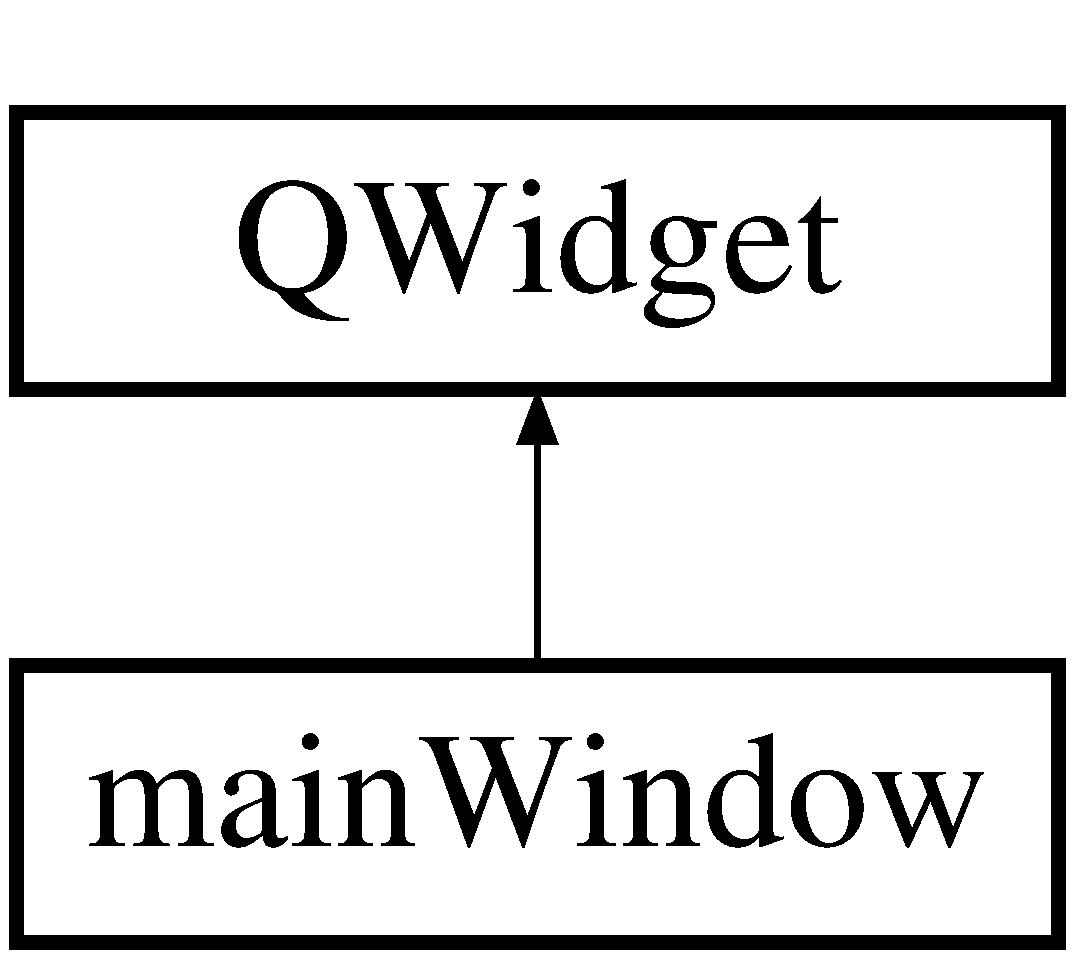
\includegraphics[height=2.000000cm]{classmain_window}
\end{center}
\end{figure}
\subsection*{Public Slots}
\begin{DoxyCompactItemize}
\item 
void \hyperlink{classmain_window_ae38f3474108e081d12b5c2bafd09714b}{take\+Ip} ()
\begin{DoxyCompactList}\small\item\em ? \end{DoxyCompactList}\end{DoxyCompactItemize}
\subsection*{Public Member Functions}
\begin{DoxyCompactItemize}
\item 
\hyperlink{classmain_window_a467ea0d8090c122e5b5fd69f77ed3476}{main\+Window} ()
\begin{DoxyCompactList}\small\item\em ? \end{DoxyCompactList}\end{DoxyCompactItemize}


\subsection{Detailed Description}
Class representing the QT interface. 

This class handle the interface 

\subsection{Constructor \& Destructor Documentation}
\mbox{\Hypertarget{classmain_window_a467ea0d8090c122e5b5fd69f77ed3476}\label{classmain_window_a467ea0d8090c122e5b5fd69f77ed3476}} 
\index{main\+Window@{main\+Window}!main\+Window@{main\+Window}}
\index{main\+Window@{main\+Window}!main\+Window@{main\+Window}}
\subsubsection{\texorpdfstring{main\+Window()}{mainWindow()}}
{\footnotesize\ttfamily main\+Window\+::main\+Window (\begin{DoxyParamCaption}{ }\end{DoxyParamCaption})}



? 


\begin{DoxyParams}{Parameters}
{\em void} & \\
\hline
\end{DoxyParams}


\subsection{Member Function Documentation}
\mbox{\Hypertarget{classmain_window_ae38f3474108e081d12b5c2bafd09714b}\label{classmain_window_ae38f3474108e081d12b5c2bafd09714b}} 
\index{main\+Window@{main\+Window}!take\+Ip@{take\+Ip}}
\index{take\+Ip@{take\+Ip}!main\+Window@{main\+Window}}
\subsubsection{\texorpdfstring{take\+Ip}{takeIp}}
{\footnotesize\ttfamily void main\+Window\+::take\+Ip (\begin{DoxyParamCaption}{ }\end{DoxyParamCaption})\hspace{0.3cm}{\ttfamily [slot]}}



? 


\begin{DoxyParams}{Parameters}
{\em void} & \\
\hline
\end{DoxyParams}


The documentation for this class was generated from the following files\+:\begin{DoxyCompactItemize}
\item 
client\+\_\+interface/include/mainwindow.\+h\item 
client\+\_\+interface/mainwindow.\+cpp\end{DoxyCompactItemize}

\hypertarget{class_ui_1_1_main_window}{}\section{Ui\+:\+:Main\+Window Class Reference}
\label{class_ui_1_1_main_window}\index{Ui\+::\+Main\+Window@{Ui\+::\+Main\+Window}}
Inheritance diagram for Ui\+:\+:Main\+Window\+:\begin{figure}[H]
\begin{center}
\leavevmode
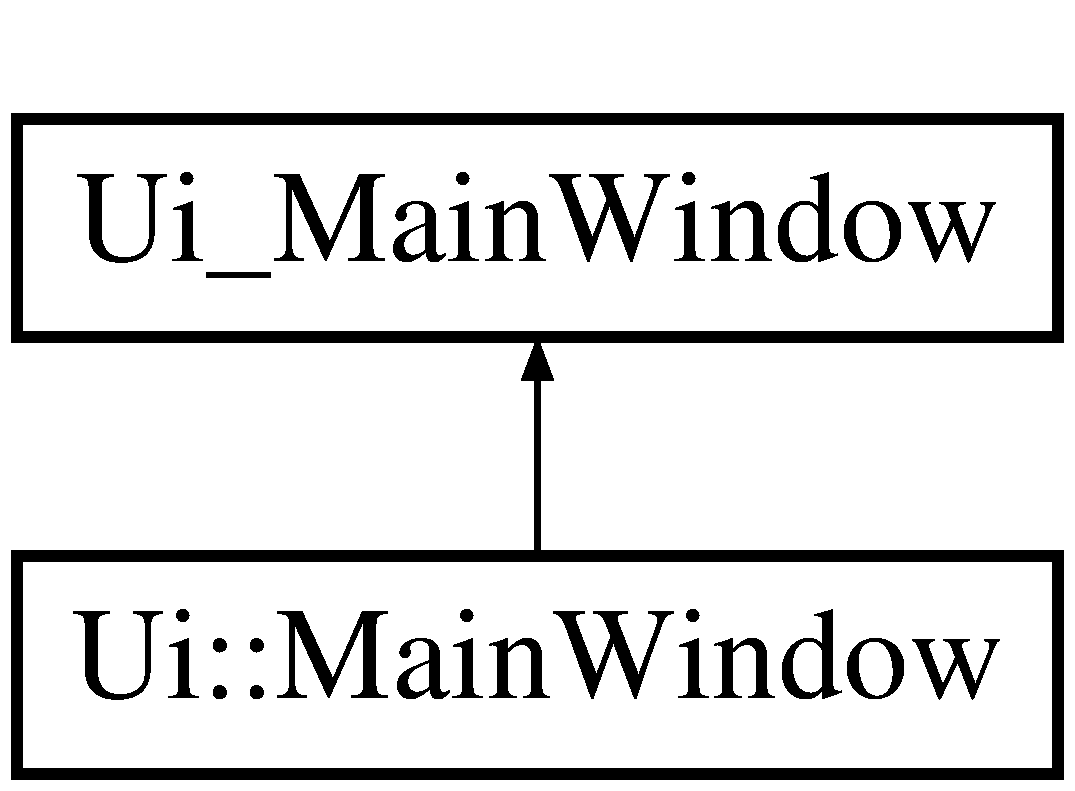
\includegraphics[height=2.000000cm]{class_ui_1_1_main_window}
\end{center}
\end{figure}
\subsection*{Additional Inherited Members}


The documentation for this class was generated from the following file\+:\begin{DoxyCompactItemize}
\item 
client\+\_\+interface/interface\+\_\+autogen/include/ui\+\_\+mainwindow.\+h\end{DoxyCompactItemize}

\hypertarget{classutils_1_1_packet}{}\section{utils\+:\+:Packet Class Reference}
\label{classutils_1_1_packet}\index{utils\+::\+Packet@{utils\+::\+Packet}}
\subsection*{Public Member Functions}
\begin{DoxyCompactItemize}
\item 
\mbox{\Hypertarget{classutils_1_1_packet_a2b59afcf9052ea39f4fbc0b3543f04f0}\label{classutils_1_1_packet_a2b59afcf9052ea39f4fbc0b3543f04f0}} 
std\+::string const {\bfseries get\+Packet} () noexcept
\item 
\mbox{\Hypertarget{classutils_1_1_packet_abf5ca12195881bf83252459b1243b1ae}\label{classutils_1_1_packet_abf5ca12195881bf83252459b1243b1ae}} 
void {\bfseries set\+Type} (const std\+::string)
\item 
\mbox{\Hypertarget{classutils_1_1_packet_aca48ed11345a8a34847fa518411b8e03}\label{classutils_1_1_packet_aca48ed11345a8a34847fa518411b8e03}} 
{\footnotesize template$<$typename T $>$ }\\void {\bfseries add\+Data} (const std\+::string name, const T data)
\item 
\mbox{\Hypertarget{classutils_1_1_packet_a484ff550a5ed540109274819b779e4f8}\label{classutils_1_1_packet_a484ff550a5ed540109274819b779e4f8}} 
{\footnotesize template$<$typename T $>$ }\\void {\bfseries add\+To\+Vector} (const T data)
\item 
\mbox{\Hypertarget{classutils_1_1_packet_a9eb149a9ee7e34e43efd04309222f765}\label{classutils_1_1_packet_a9eb149a9ee7e34e43efd04309222f765}} 
std\+::vector$<$ std\+::array$<$ float, 2 $>$ $>$ {\bfseries get\+Vector} () const noexcept
\item 
\mbox{\Hypertarget{classutils_1_1_packet_a295d6f0e6e90db9c0e2647b4f6ffe93b}\label{classutils_1_1_packet_a295d6f0e6e90db9c0e2647b4f6ffe93b}} 
std\+::size\+\_\+t {\bfseries get\+Vector\+Size} () const noexcept
\item 
\mbox{\Hypertarget{classutils_1_1_packet_aba28b71a578335ed5ebdacb9660ac6c5}\label{classutils_1_1_packet_aba28b71a578335ed5ebdacb9660ac6c5}} 
{\footnotesize template$<$typename T $>$ }\\void {\bfseries add\+Pair\+To\+List} (const std\+::string name1, const std\+::string name2, T elem1, T elem2)
\item 
\mbox{\Hypertarget{classutils_1_1_packet_a7e60a3b763cda5855003bb36603fa73e}\label{classutils_1_1_packet_a7e60a3b763cda5855003bb36603fa73e}} 
{\footnotesize template$<$typename T $>$ }\\void {\bfseries add\+Data\+To\+List} (const std\+::string name, const T data)
\item 
\mbox{\Hypertarget{classutils_1_1_packet_acbe9279b935384537850daa1b9a8c982}\label{classutils_1_1_packet_acbe9279b935384537850daa1b9a8c982}} 
{\footnotesize template$<$typename T $>$ }\\void {\bfseries add\+List} (const std\+::string name, std\+::vector$<$ T $>$ data)
\item 
\mbox{\Hypertarget{classutils_1_1_packet_a583c5366ba6e32d1a4df8cb491e6dcd4}\label{classutils_1_1_packet_a583c5366ba6e32d1a4df8cb491e6dcd4}} 
void {\bfseries clear} ()
\end{DoxyCompactItemize}


The documentation for this class was generated from the following files\+:\begin{DoxyCompactItemize}
\item 
utils/include/Packet.\+hpp\item 
utils/srcs/Packet.\+cpp\end{DoxyCompactItemize}

\hypertarget{structpa_test_data}{}\section{pa\+Test\+Data Struct Reference}
\label{structpa_test_data}\index{pa\+Test\+Data@{pa\+Test\+Data}}
\subsection*{Public Attributes}
\begin{DoxyCompactItemize}
\item 
\mbox{\Hypertarget{structpa_test_data_ab6998ce9ea16a1cbfd92239f9db30091}\label{structpa_test_data_ab6998ce9ea16a1cbfd92239f9db30091}} 
int {\bfseries frame\+Index}
\item 
\mbox{\Hypertarget{structpa_test_data_af927cb4284f8d465356704d60690fba5}\label{structpa_test_data_af927cb4284f8d465356704d60690fba5}} 
int {\bfseries max\+Frame\+Index}
\item 
\mbox{\Hypertarget{structpa_test_data_a7d998f00d501e39a7ef025d79d6f918a}\label{structpa_test_data_a7d998f00d501e39a7ef025d79d6f918a}} 
float $\ast$ {\bfseries recorded\+Samples}
\end{DoxyCompactItemize}


The documentation for this struct was generated from the following file\+:\begin{DoxyCompactItemize}
\item 
audio/include/Port\+Audio.\+hpp\end{DoxyCompactItemize}

\hypertarget{class_port_audio}{}\section{Port\+Audio Class Reference}
\label{class_port_audio}\index{Port\+Audio@{Port\+Audio}}
\subsection*{Public Member Functions}
\begin{DoxyCompactItemize}
\item 
\hyperlink{class_port_audio_ad5640eccbb52a46880bf424f26d1809f}{Port\+Audio} ()
\begin{DoxyCompactList}\small\item\em ? \end{DoxyCompactList}\item 
\hyperlink{class_port_audio_a5f80fdff2377981fcd42fae42d4b65c3}{$\sim$\+Port\+Audio} ()
\begin{DoxyCompactList}\small\item\em ? \end{DoxyCompactList}\item 
void \hyperlink{class_port_audio_aba9d07307c1d1da76f60b34c36e7b307}{Set\+Input\+Parameters} ()
\begin{DoxyCompactList}\small\item\em ? \end{DoxyCompactList}\item 
void \hyperlink{class_port_audio_ab6c65dcf34b99509ef98eb6025f3f2c9}{Set\+Output\+Parameters} ()
\begin{DoxyCompactList}\small\item\em ? \end{DoxyCompactList}\item 
void \hyperlink{class_port_audio_adbe0192928bae24d0d469b39561b9859}{Set\+Data} (int, int, int)
\begin{DoxyCompactList}\small\item\em ? \end{DoxyCompactList}\item 
void \hyperlink{class_port_audio_a0da7ed31a1a6e38800c4f4e2e179565f}{Start\+Stream} (Pa\+Stream $\ast$)
\begin{DoxyCompactList}\small\item\em ? \end{DoxyCompactList}\item 
void \hyperlink{class_port_audio_acb0f54f9382bc8da31d2a39bcf88bb36}{Close\+Stream} (Pa\+Stream $\ast$)
\begin{DoxyCompactList}\small\item\em ? \end{DoxyCompactList}\item 
Pa\+Stream $\ast$ \hyperlink{class_port_audio_a0096f886eec6c33ae24b4610f9ee3fcb}{Record\+Stream} ()
\begin{DoxyCompactList}\small\item\em ? \end{DoxyCompactList}\item 
void \hyperlink{class_port_audio_ac3d84aa081e68ed4b6b32e901a25ea8c}{Play\+Stream} (Pa\+Stream $\ast$)
\begin{DoxyCompactList}\small\item\em ? \end{DoxyCompactList}\item 
void \hyperlink{class_port_audio_a8d6e5890ce34df315cbb76b2399d1876}{set\+Sample\+Rate} (short)
\begin{DoxyCompactList}\small\item\em ? \end{DoxyCompactList}\item 
void \hyperlink{class_port_audio_ad86fa6db404b8f563b7eb92c1b4359b5}{set\+Frame\+Per\+Buffer} (short)
\begin{DoxyCompactList}\small\item\em ? \end{DoxyCompactList}\item 
void \hyperlink{class_port_audio_a42e4b5882022a7ccd8696d9656ea686d}{set\+Data\+Frame\+Index} ()
\begin{DoxyCompactList}\small\item\em ? \end{DoxyCompactList}\end{DoxyCompactItemize}


\subsection{Constructor \& Destructor Documentation}
\mbox{\Hypertarget{class_port_audio_ad5640eccbb52a46880bf424f26d1809f}\label{class_port_audio_ad5640eccbb52a46880bf424f26d1809f}} 
\index{Port\+Audio@{Port\+Audio}!Port\+Audio@{Port\+Audio}}
\index{Port\+Audio@{Port\+Audio}!Port\+Audio@{Port\+Audio}}
\subsubsection{\texorpdfstring{Port\+Audio()}{PortAudio()}}
{\footnotesize\ttfamily Port\+Audio\+::\+Port\+Audio (\begin{DoxyParamCaption}{ }\end{DoxyParamCaption})}



? 


\begin{DoxyParams}{Parameters}
{\em void} & \\
\hline
\end{DoxyParams}
\mbox{\Hypertarget{class_port_audio_a5f80fdff2377981fcd42fae42d4b65c3}\label{class_port_audio_a5f80fdff2377981fcd42fae42d4b65c3}} 
\index{Port\+Audio@{Port\+Audio}!````~Port\+Audio@{$\sim$\+Port\+Audio}}
\index{````~Port\+Audio@{$\sim$\+Port\+Audio}!Port\+Audio@{Port\+Audio}}
\subsubsection{\texorpdfstring{$\sim$\+Port\+Audio()}{~PortAudio()}}
{\footnotesize\ttfamily Port\+Audio\+::$\sim$\+Port\+Audio (\begin{DoxyParamCaption}{ }\end{DoxyParamCaption})}



? 


\begin{DoxyParams}{Parameters}
{\em void} & \\
\hline
\end{DoxyParams}


\subsection{Member Function Documentation}
\mbox{\Hypertarget{class_port_audio_acb0f54f9382bc8da31d2a39bcf88bb36}\label{class_port_audio_acb0f54f9382bc8da31d2a39bcf88bb36}} 
\index{Port\+Audio@{Port\+Audio}!Close\+Stream@{Close\+Stream}}
\index{Close\+Stream@{Close\+Stream}!Port\+Audio@{Port\+Audio}}
\subsubsection{\texorpdfstring{Close\+Stream()}{CloseStream()}}
{\footnotesize\ttfamily void Port\+Audio\+::\+Close\+Stream (\begin{DoxyParamCaption}\item[{Pa\+Stream $\ast$}]{stream }\end{DoxyParamCaption})}



? 


\begin{DoxyParams}{Parameters}
{\em Pa\+Stream} & $\ast$stream \\
\hline
\end{DoxyParams}
\mbox{\Hypertarget{class_port_audio_ac3d84aa081e68ed4b6b32e901a25ea8c}\label{class_port_audio_ac3d84aa081e68ed4b6b32e901a25ea8c}} 
\index{Port\+Audio@{Port\+Audio}!Play\+Stream@{Play\+Stream}}
\index{Play\+Stream@{Play\+Stream}!Port\+Audio@{Port\+Audio}}
\subsubsection{\texorpdfstring{Play\+Stream()}{PlayStream()}}
{\footnotesize\ttfamily void Port\+Audio\+::\+Play\+Stream (\begin{DoxyParamCaption}\item[{Pa\+Stream $\ast$}]{stream }\end{DoxyParamCaption})}



? 


\begin{DoxyParams}{Parameters}
{\em Pa\+Stream} & $\ast$stream \\
\hline
\end{DoxyParams}
\mbox{\Hypertarget{class_port_audio_a0096f886eec6c33ae24b4610f9ee3fcb}\label{class_port_audio_a0096f886eec6c33ae24b4610f9ee3fcb}} 
\index{Port\+Audio@{Port\+Audio}!Record\+Stream@{Record\+Stream}}
\index{Record\+Stream@{Record\+Stream}!Port\+Audio@{Port\+Audio}}
\subsubsection{\texorpdfstring{Record\+Stream()}{RecordStream()}}
{\footnotesize\ttfamily Pa\+Stream $\ast$ Port\+Audio\+::\+Record\+Stream (\begin{DoxyParamCaption}{ }\end{DoxyParamCaption})}



? 


\begin{DoxyParams}{Parameters}
{\em void} & \\
\hline
\end{DoxyParams}
\mbox{\Hypertarget{class_port_audio_adbe0192928bae24d0d469b39561b9859}\label{class_port_audio_adbe0192928bae24d0d469b39561b9859}} 
\index{Port\+Audio@{Port\+Audio}!Set\+Data@{Set\+Data}}
\index{Set\+Data@{Set\+Data}!Port\+Audio@{Port\+Audio}}
\subsubsection{\texorpdfstring{Set\+Data()}{SetData()}}
{\footnotesize\ttfamily void Port\+Audio\+::\+Set\+Data (\begin{DoxyParamCaption}\item[{int}]{num\+\_\+seconds,  }\item[{int}]{sample\+\_\+rate,  }\item[{int}]{num\+\_\+channels }\end{DoxyParamCaption})}



? 


\begin{DoxyParams}{Parameters}
{\em int} & num\+\_\+seconds, int sample\+\_\+rate, int num\+\_\+channels \\
\hline
\end{DoxyParams}
\mbox{\Hypertarget{class_port_audio_a42e4b5882022a7ccd8696d9656ea686d}\label{class_port_audio_a42e4b5882022a7ccd8696d9656ea686d}} 
\index{Port\+Audio@{Port\+Audio}!set\+Data\+Frame\+Index@{set\+Data\+Frame\+Index}}
\index{set\+Data\+Frame\+Index@{set\+Data\+Frame\+Index}!Port\+Audio@{Port\+Audio}}
\subsubsection{\texorpdfstring{set\+Data\+Frame\+Index()}{setDataFrameIndex()}}
{\footnotesize\ttfamily void Port\+Audio\+::set\+Data\+Frame\+Index (\begin{DoxyParamCaption}{ }\end{DoxyParamCaption})}



? 


\begin{DoxyParams}{Parameters}
{\em void} & \\
\hline
\end{DoxyParams}
\mbox{\Hypertarget{class_port_audio_ad86fa6db404b8f563b7eb92c1b4359b5}\label{class_port_audio_ad86fa6db404b8f563b7eb92c1b4359b5}} 
\index{Port\+Audio@{Port\+Audio}!set\+Frame\+Per\+Buffer@{set\+Frame\+Per\+Buffer}}
\index{set\+Frame\+Per\+Buffer@{set\+Frame\+Per\+Buffer}!Port\+Audio@{Port\+Audio}}
\subsubsection{\texorpdfstring{set\+Frame\+Per\+Buffer()}{setFramePerBuffer()}}
{\footnotesize\ttfamily void Port\+Audio\+::set\+Frame\+Per\+Buffer (\begin{DoxyParamCaption}\item[{short}]{frame\+\_\+per\+\_\+buffer }\end{DoxyParamCaption})}



? 


\begin{DoxyParams}{Parameters}
{\em short} & frame\+\_\+per\+\_\+buffer \\
\hline
\end{DoxyParams}
\mbox{\Hypertarget{class_port_audio_aba9d07307c1d1da76f60b34c36e7b307}\label{class_port_audio_aba9d07307c1d1da76f60b34c36e7b307}} 
\index{Port\+Audio@{Port\+Audio}!Set\+Input\+Parameters@{Set\+Input\+Parameters}}
\index{Set\+Input\+Parameters@{Set\+Input\+Parameters}!Port\+Audio@{Port\+Audio}}
\subsubsection{\texorpdfstring{Set\+Input\+Parameters()}{SetInputParameters()}}
{\footnotesize\ttfamily void Port\+Audio\+::\+Set\+Input\+Parameters (\begin{DoxyParamCaption}{ }\end{DoxyParamCaption})}



? 


\begin{DoxyParams}{Parameters}
{\em void} & \\
\hline
\end{DoxyParams}
\mbox{\Hypertarget{class_port_audio_ab6c65dcf34b99509ef98eb6025f3f2c9}\label{class_port_audio_ab6c65dcf34b99509ef98eb6025f3f2c9}} 
\index{Port\+Audio@{Port\+Audio}!Set\+Output\+Parameters@{Set\+Output\+Parameters}}
\index{Set\+Output\+Parameters@{Set\+Output\+Parameters}!Port\+Audio@{Port\+Audio}}
\subsubsection{\texorpdfstring{Set\+Output\+Parameters()}{SetOutputParameters()}}
{\footnotesize\ttfamily void Port\+Audio\+::\+Set\+Output\+Parameters (\begin{DoxyParamCaption}{ }\end{DoxyParamCaption})}



? 


\begin{DoxyParams}{Parameters}
{\em void} & \\
\hline
\end{DoxyParams}
\mbox{\Hypertarget{class_port_audio_a8d6e5890ce34df315cbb76b2399d1876}\label{class_port_audio_a8d6e5890ce34df315cbb76b2399d1876}} 
\index{Port\+Audio@{Port\+Audio}!set\+Sample\+Rate@{set\+Sample\+Rate}}
\index{set\+Sample\+Rate@{set\+Sample\+Rate}!Port\+Audio@{Port\+Audio}}
\subsubsection{\texorpdfstring{set\+Sample\+Rate()}{setSampleRate()}}
{\footnotesize\ttfamily void Port\+Audio\+::set\+Sample\+Rate (\begin{DoxyParamCaption}\item[{short}]{sample\+\_\+rate }\end{DoxyParamCaption})}



? 


\begin{DoxyParams}{Parameters}
{\em short} & sample\+\_\+rate \\
\hline
\end{DoxyParams}
\mbox{\Hypertarget{class_port_audio_a0da7ed31a1a6e38800c4f4e2e179565f}\label{class_port_audio_a0da7ed31a1a6e38800c4f4e2e179565f}} 
\index{Port\+Audio@{Port\+Audio}!Start\+Stream@{Start\+Stream}}
\index{Start\+Stream@{Start\+Stream}!Port\+Audio@{Port\+Audio}}
\subsubsection{\texorpdfstring{Start\+Stream()}{StartStream()}}
{\footnotesize\ttfamily void Port\+Audio\+::\+Start\+Stream (\begin{DoxyParamCaption}\item[{Pa\+Stream $\ast$}]{stream }\end{DoxyParamCaption})}



? 


\begin{DoxyParams}{Parameters}
{\em Pa\+Stream} & $\ast$stream \\
\hline
\end{DoxyParams}


The documentation for this class was generated from the following files\+:\begin{DoxyCompactItemize}
\item 
audio/include/Port\+Audio.\+hpp\item 
audio/srcs/Port\+Audio.\+cpp\end{DoxyCompactItemize}

\hypertarget{structcli_1_1props__s}{}\section{cli\+:\+:props\+\_\+s Struct Reference}
\label{structcli_1_1props__s}\index{cli\+::props\+\_\+s@{cli\+::props\+\_\+s}}
\subsection*{Public Attributes}
\begin{DoxyCompactItemize}
\item 
\mbox{\Hypertarget{structcli_1_1props__s_ab3a14790c469e94078653826c8ac41b3}\label{structcli_1_1props__s_ab3a14790c469e94078653826c8ac41b3}} 
std\+::string {\bfseries username}
\item 
\mbox{\Hypertarget{structcli_1_1props__s_a82273ac86c113554ee891c5fa4bf8243}\label{structcli_1_1props__s_a82273ac86c113554ee891c5fa4bf8243}} 
\hyperlink{class_t_c_p_socket}{T\+C\+P\+Socket} {\bfseries socket}
\end{DoxyCompactItemize}


The documentation for this struct was generated from the following file\+:\begin{DoxyCompactItemize}
\item 
network/include/Client.\+hpp\end{DoxyCompactItemize}

\hypertarget{structqt__meta__stringdata__main_window__t}{}\section{qt\+\_\+meta\+\_\+stringdata\+\_\+main\+Window\+\_\+t Struct Reference}
\label{structqt__meta__stringdata__main_window__t}\index{qt\+\_\+meta\+\_\+stringdata\+\_\+main\+Window\+\_\+t@{qt\+\_\+meta\+\_\+stringdata\+\_\+main\+Window\+\_\+t}}
\subsection*{Public Attributes}
\begin{DoxyCompactItemize}
\item 
\mbox{\Hypertarget{structqt__meta__stringdata__main_window__t_ab43a3a6dea57c7e0704a00eb4871ed37}\label{structqt__meta__stringdata__main_window__t_ab43a3a6dea57c7e0704a00eb4871ed37}} 
Q\+Byte\+Array\+Data {\bfseries data} \mbox{[}3\mbox{]}
\item 
\mbox{\Hypertarget{structqt__meta__stringdata__main_window__t_a15c5ced06463db8cc0a06eee1d44f22d}\label{structqt__meta__stringdata__main_window__t_a15c5ced06463db8cc0a06eee1d44f22d}} 
char {\bfseries stringdata0} \mbox{[}19\mbox{]}
\end{DoxyCompactItemize}


The documentation for this struct was generated from the following file\+:\begin{DoxyCompactItemize}
\item 
client\+\_\+interface/include/moc\+\_\+mainwindow.\+cpp\end{DoxyCompactItemize}

\hypertarget{class_server}{}\section{Server Class Reference}
\label{class_server}\index{Server@{Server}}


Class representing the \hyperlink{class_server}{Server}.  




{\ttfamily \#include $<$Server.\+hpp$>$}



\subsection{Detailed Description}
Class representing the \hyperlink{class_server}{Server}. 

This class handle of the logic of the program, it loads the libraires and the protocols it can switch at any given moments 

The documentation for this class was generated from the following file\+:\begin{DoxyCompactItemize}
\item 
network/include/Server.\+hpp\end{DoxyCompactItemize}

\hypertarget{classns_1_1_server}{}\section{ns\+:\+:Server Class Reference}
\label{classns_1_1_server}\index{ns\+::\+Server@{ns\+::\+Server}}
Inheritance diagram for ns\+:\+:Server\+:\begin{figure}[H]
\begin{center}
\leavevmode
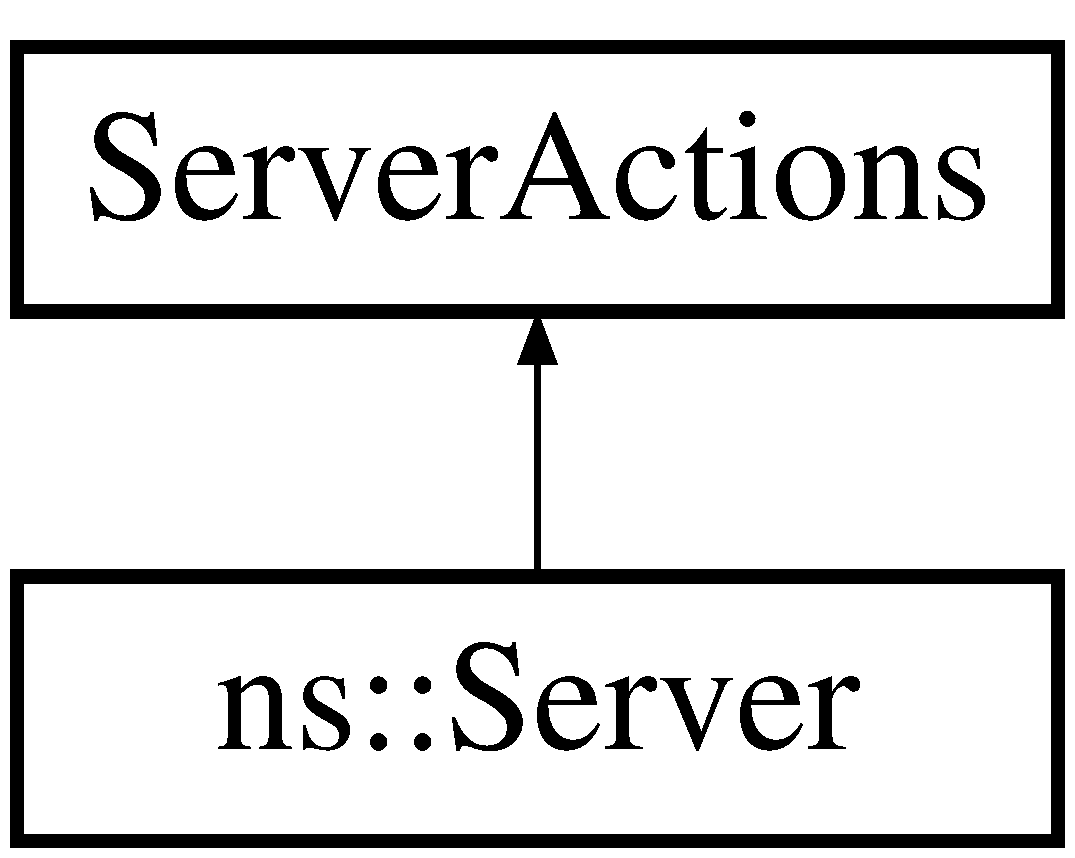
\includegraphics[height=2.000000cm]{classns_1_1_server}
\end{center}
\end{figure}
\subsection*{Public Member Functions}
\begin{DoxyCompactItemize}
\item 
\hyperlink{classns_1_1_server_a349ed2f3b045602da2f1b9b91a11b78c}{Server} (const int port)
\begin{DoxyCompactList}\small\item\em Open connection with port in param. \end{DoxyCompactList}\item 
\hyperlink{classns_1_1_server_a4b3aa2579cb1c8cd1d069582c14d0fa6}{$\sim$\+Server} ()
\begin{DoxyCompactList}\small\item\em Destroy the \hyperlink{classns_1_1_server}{Server} by reseting the shared pointers. \end{DoxyCompactList}\item 
void \hyperlink{classns_1_1_server_a101fc02efc9caec89146f34619c03e95}{remove\+Client} (\hyperlink{class_server_client}{Server\+Client})
\begin{DoxyCompactList}\small\item\em remove pecno \end{DoxyCompactList}\item 
void \hyperlink{classns_1_1_server_a9e8e68bd5147b294ed9a0d23c1189f6d}{Poll\+Event} ()
\begin{DoxyCompactList}\small\item\em Poll the event. \end{DoxyCompactList}\item 
void \hyperlink{classns_1_1_server_ac0ac436c081e25c992d2b6dd1632ff71}{Run} ()
\begin{DoxyCompactList}\small\item\em Run the server. \end{DoxyCompactList}\item 
\mbox{\Hypertarget{classns_1_1_server_abf2a4da899c012d24a89a003fc2b3366}\label{classns_1_1_server_abf2a4da899c012d24a89a003fc2b3366}} 
void {\bfseries shutdown} ()
\item 
void \hyperlink{classns_1_1_server_add5a181b9d70456b7e80cb258f32b8fd}{Handle\+Connection} ()
\begin{DoxyCompactList}\small\item\em Handle connection. \end{DoxyCompactList}\item 
void \hyperlink{classns_1_1_server_ad1d8a69bcfb01d6a13a05afe6a4de7cb}{Handle\+Receive} (\hyperlink{class_server_client}{Server\+Client})
\begin{DoxyCompactList}\small\item\em Handle receive. \end{DoxyCompactList}\item 
bool \hyperlink{classns_1_1_server_a8b83ee853238667ba56c4bb1f064364e}{update\+Database} (client\+\_\+p)
\begin{DoxyCompactList}\small\item\em updtae database \end{DoxyCompactList}\item 
void \hyperlink{classns_1_1_server_a99e12a7ee8a2bc21ada58e6870990189}{Match\+Command} (client\+\_\+p client, const std\+::string \&command)
\begin{DoxyCompactList}\small\item\em Match command. \end{DoxyCompactList}\item 
\mbox{\Hypertarget{classns_1_1_server_a1f8c4e0dd82588f988427c5ff0de4832}\label{classns_1_1_server_a1f8c4e0dd82588f988427c5ff0de4832}} 
void {\bfseries Call} (client\+\_\+p client)
\end{DoxyCompactItemize}


\subsection{Constructor \& Destructor Documentation}
\mbox{\Hypertarget{classns_1_1_server_a349ed2f3b045602da2f1b9b91a11b78c}\label{classns_1_1_server_a349ed2f3b045602da2f1b9b91a11b78c}} 
\index{ns\+::\+Server@{ns\+::\+Server}!Server@{Server}}
\index{Server@{Server}!ns\+::\+Server@{ns\+::\+Server}}
\subsubsection{\texorpdfstring{Server()}{Server()}}
{\footnotesize\ttfamily Server\+::\+Server (\begin{DoxyParamCaption}\item[{const int}]{port = {\ttfamily DEFAULT\+\_\+PORT} }\end{DoxyParamCaption})}



Open connection with port in param. 


\begin{DoxyParams}{Parameters}
{\em int} & port representing the port \\
\hline
\end{DoxyParams}
\mbox{\Hypertarget{classns_1_1_server_a4b3aa2579cb1c8cd1d069582c14d0fa6}\label{classns_1_1_server_a4b3aa2579cb1c8cd1d069582c14d0fa6}} 
\index{ns\+::\+Server@{ns\+::\+Server}!````~Server@{$\sim$\+Server}}
\index{````~Server@{$\sim$\+Server}!ns\+::\+Server@{ns\+::\+Server}}
\subsubsection{\texorpdfstring{$\sim$\+Server()}{~Server()}}
{\footnotesize\ttfamily Server\+::$\sim$\+Server (\begin{DoxyParamCaption}{ }\end{DoxyParamCaption})}



Destroy the \hyperlink{classns_1_1_server}{Server} by reseting the shared pointers. 


\begin{DoxyParams}{Parameters}
{\em void} & \\
\hline
\end{DoxyParams}


\subsection{Member Function Documentation}
\mbox{\Hypertarget{classns_1_1_server_add5a181b9d70456b7e80cb258f32b8fd}\label{classns_1_1_server_add5a181b9d70456b7e80cb258f32b8fd}} 
\index{ns\+::\+Server@{ns\+::\+Server}!Handle\+Connection@{Handle\+Connection}}
\index{Handle\+Connection@{Handle\+Connection}!ns\+::\+Server@{ns\+::\+Server}}
\subsubsection{\texorpdfstring{Handle\+Connection()}{HandleConnection()}}
{\footnotesize\ttfamily void Server\+::\+Handle\+Connection (\begin{DoxyParamCaption}{ }\end{DoxyParamCaption})}



Handle connection. 


\begin{DoxyParams}{Parameters}
{\em void} & \\
\hline
\end{DoxyParams}
\mbox{\Hypertarget{classns_1_1_server_ad1d8a69bcfb01d6a13a05afe6a4de7cb}\label{classns_1_1_server_ad1d8a69bcfb01d6a13a05afe6a4de7cb}} 
\index{ns\+::\+Server@{ns\+::\+Server}!Handle\+Receive@{Handle\+Receive}}
\index{Handle\+Receive@{Handle\+Receive}!ns\+::\+Server@{ns\+::\+Server}}
\subsubsection{\texorpdfstring{Handle\+Receive()}{HandleReceive()}}
{\footnotesize\ttfamily void Server\+::\+Handle\+Receive (\begin{DoxyParamCaption}\item[{\hyperlink{class_server_client}{Server\+Client}}]{client }\end{DoxyParamCaption})}



Handle receive. 


\begin{DoxyParams}{Parameters}
{\em \hyperlink{class_server_client}{Server\+Client}} & client \\
\hline
\end{DoxyParams}
\mbox{\Hypertarget{classns_1_1_server_a99e12a7ee8a2bc21ada58e6870990189}\label{classns_1_1_server_a99e12a7ee8a2bc21ada58e6870990189}} 
\index{ns\+::\+Server@{ns\+::\+Server}!Match\+Command@{Match\+Command}}
\index{Match\+Command@{Match\+Command}!ns\+::\+Server@{ns\+::\+Server}}
\subsubsection{\texorpdfstring{Match\+Command()}{MatchCommand()}}
{\footnotesize\ttfamily void Server\+::\+Match\+Command (\begin{DoxyParamCaption}\item[{client\+\_\+p}]{client,  }\item[{const std\+::string \&}]{packet }\end{DoxyParamCaption})}



Match command. 


\begin{DoxyParams}{Parameters}
{\em client\+\_\+p} & client, const std\+::string \&packet \\
\hline
\end{DoxyParams}
\mbox{\Hypertarget{classns_1_1_server_a9e8e68bd5147b294ed9a0d23c1189f6d}\label{classns_1_1_server_a9e8e68bd5147b294ed9a0d23c1189f6d}} 
\index{ns\+::\+Server@{ns\+::\+Server}!Poll\+Event@{Poll\+Event}}
\index{Poll\+Event@{Poll\+Event}!ns\+::\+Server@{ns\+::\+Server}}
\subsubsection{\texorpdfstring{Poll\+Event()}{PollEvent()}}
{\footnotesize\ttfamily void Server\+::\+Poll\+Event (\begin{DoxyParamCaption}{ }\end{DoxyParamCaption})}



Poll the event. 


\begin{DoxyParams}{Parameters}
{\em void} & \\
\hline
\end{DoxyParams}
\mbox{\Hypertarget{classns_1_1_server_a101fc02efc9caec89146f34619c03e95}\label{classns_1_1_server_a101fc02efc9caec89146f34619c03e95}} 
\index{ns\+::\+Server@{ns\+::\+Server}!remove\+Client@{remove\+Client}}
\index{remove\+Client@{remove\+Client}!ns\+::\+Server@{ns\+::\+Server}}
\subsubsection{\texorpdfstring{remove\+Client()}{removeClient()}}
{\footnotesize\ttfamily void Server\+::remove\+Client (\begin{DoxyParamCaption}\item[{\hyperlink{class_server_client}{Server\+Client}}]{client }\end{DoxyParamCaption})}



remove pecno 


\begin{DoxyParams}{Parameters}
{\em \hyperlink{class_server_client}{Server\+Client}} & client \\
\hline
\end{DoxyParams}
\mbox{\Hypertarget{classns_1_1_server_ac0ac436c081e25c992d2b6dd1632ff71}\label{classns_1_1_server_ac0ac436c081e25c992d2b6dd1632ff71}} 
\index{ns\+::\+Server@{ns\+::\+Server}!Run@{Run}}
\index{Run@{Run}!ns\+::\+Server@{ns\+::\+Server}}
\subsubsection{\texorpdfstring{Run()}{Run()}}
{\footnotesize\ttfamily void Server\+::\+Run (\begin{DoxyParamCaption}{ }\end{DoxyParamCaption})}



Run the server. 


\begin{DoxyParams}{Parameters}
{\em void} & \\
\hline
\end{DoxyParams}
\mbox{\Hypertarget{classns_1_1_server_a8b83ee853238667ba56c4bb1f064364e}\label{classns_1_1_server_a8b83ee853238667ba56c4bb1f064364e}} 
\index{ns\+::\+Server@{ns\+::\+Server}!update\+Database@{update\+Database}}
\index{update\+Database@{update\+Database}!ns\+::\+Server@{ns\+::\+Server}}
\subsubsection{\texorpdfstring{update\+Database()}{updateDatabase()}}
{\footnotesize\ttfamily bool Server\+::update\+Database (\begin{DoxyParamCaption}\item[{client\+\_\+p}]{client }\end{DoxyParamCaption})}



updtae database 


\begin{DoxyParams}{Parameters}
{\em client\+\_\+p} & client \\
\hline
\end{DoxyParams}


The documentation for this class was generated from the following files\+:\begin{DoxyCompactItemize}
\item 
network/include/Server.\+hpp\item 
network/server/server.\+cpp\end{DoxyCompactItemize}

\hypertarget{class_server_actions}{}\section{Server\+Actions Class Reference}
\label{class_server_actions}\index{Server\+Actions@{Server\+Actions}}


Class representing the \hyperlink{class_server_actions}{Server\+Actions}.  




{\ttfamily \#include $<$Server\+Actions.\+hpp$>$}

Inheritance diagram for Server\+Actions\+:\begin{figure}[H]
\begin{center}
\leavevmode
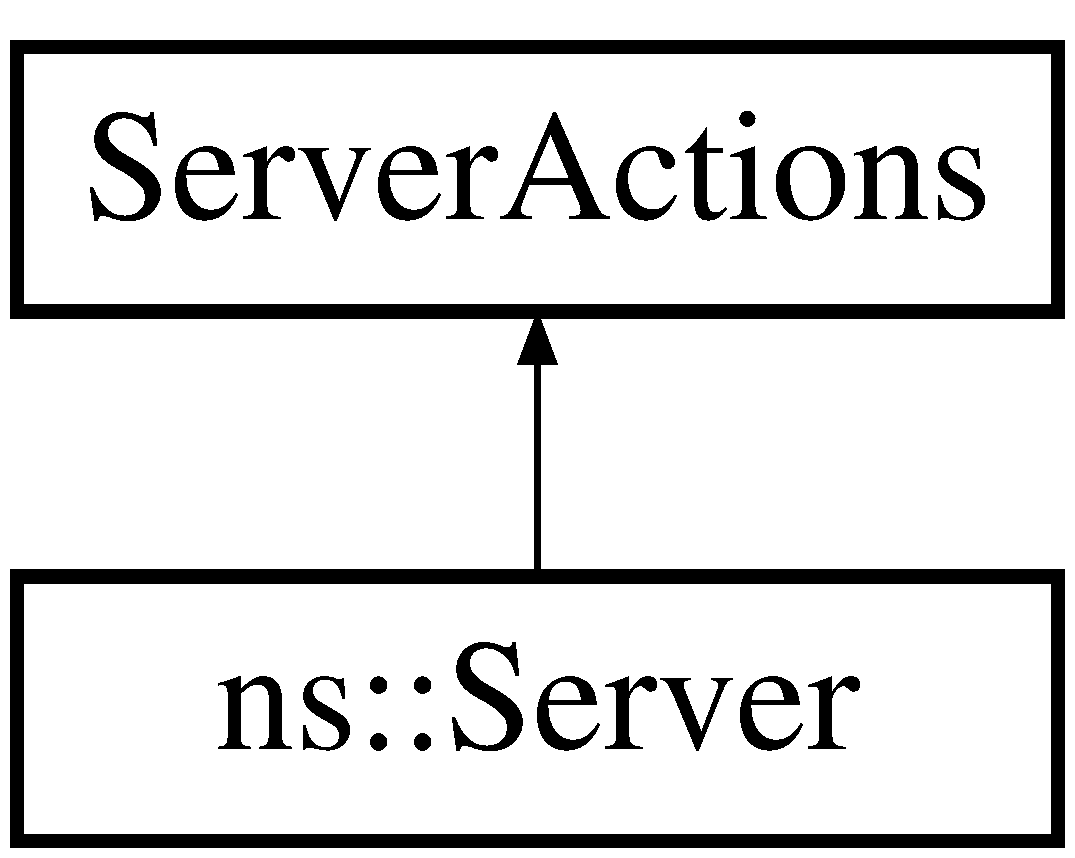
\includegraphics[height=2.000000cm]{class_server_actions}
\end{center}
\end{figure}
\subsection*{Public Member Functions}
\begin{DoxyCompactItemize}
\item 
\mbox{\Hypertarget{class_server_actions_af37fa5e3c48b269ea5c020b398a9791f}\label{class_server_actions_af37fa5e3c48b269ea5c020b398a9791f}} 
bool {\bfseries init\+Connection} (std\+::unique\+\_\+ptr$<$ \hyperlink{class_server_client}{Server\+Client} $>$)
\item 
\mbox{\Hypertarget{class_server_actions_a84b54c31a9b2c36b71e60d96c4551691}\label{class_server_actions_a84b54c31a9b2c36b71e60d96c4551691}} 
bool {\bfseries close\+Connection} (std\+::unique\+\_\+ptr$<$ \hyperlink{class_server_client}{Server\+Client} $>$)
\item 
\mbox{\Hypertarget{class_server_actions_a5010277a6ba0dcab261f6a506990a234}\label{class_server_actions_a5010277a6ba0dcab261f6a506990a234}} 
bool {\bfseries get\+Infos} (std\+::unique\+\_\+ptr$<$ \hyperlink{class_server_client}{Server\+Client} $>$)
\end{DoxyCompactItemize}


\subsection{Detailed Description}
Class representing the \hyperlink{class_server_actions}{Server\+Actions}. 

This class handle the server\textquotesingle{}s actions 

The documentation for this class was generated from the following files\+:\begin{DoxyCompactItemize}
\item 
network/include/Server\+Actions.\+hpp\item 
network/server/Server\+Actions.\+cpp\end{DoxyCompactItemize}

\hypertarget{class_server_client}{}\section{Server\+Client Class Reference}
\label{class_server_client}\index{Server\+Client@{Server\+Client}}


Class representing the \hyperlink{class_server_client}{Server\+Client}.  




{\ttfamily \#include $<$Server\+Client.\+hpp$>$}

\subsection*{Public Member Functions}
\begin{DoxyCompactItemize}
\item 
\mbox{\Hypertarget{class_server_client_a8598a1d9718e6e9b44b907c29adb6ab4}\label{class_server_client_a8598a1d9718e6e9b44b907c29adb6ab4}} 
{\bfseries Server\+Client} (\hyperlink{class_socket}{Socket} sock)
\item 
\mbox{\Hypertarget{class_server_client_a2eb72f997cdd9e2294e7ad4e4e32f83e}\label{class_server_client_a2eb72f997cdd9e2294e7ad4e4e32f83e}} 
std\+::string {\bfseries get\+Username} () const noexcept
\end{DoxyCompactItemize}
\subsection*{Public Attributes}
\begin{DoxyCompactItemize}
\item 
\mbox{\Hypertarget{class_server_client_a9aafd3f8ae06874dcad8362080f0c117}\label{class_server_client_a9aafd3f8ae06874dcad8362080f0c117}} 
\hyperlink{class_socket}{Socket} {\bfseries \+\_\+sock}
\end{DoxyCompactItemize}


\subsection{Detailed Description}
Class representing the \hyperlink{class_server_client}{Server\+Client}. 

This class handle the server\textquotesingle{}s clients 

The documentation for this class was generated from the following files\+:\begin{DoxyCompactItemize}
\item 
network/include/Server\+Client.\+hpp\item 
network/server/Server\+Client.\+cpp\end{DoxyCompactItemize}

\hypertarget{class_socket}{}\section{Socket Class Reference}
\label{class_socket}\index{Socket@{Socket}}


Class representing the \hyperlink{class_socket}{Socket}.  




{\ttfamily \#include $<$Socket.\+hpp$>$}

\subsection*{Public Member Functions}
\begin{DoxyCompactItemize}
\item 
\hyperlink{class_socket_a7c3256c4fc6e2c603df73201049fae5a}{Socket} ()
\begin{DoxyCompactList}\small\item\em Open connection. \end{DoxyCompactList}\item 
bool \hyperlink{class_socket_a6afde2dca985dacdfa770141192e2daf}{create} ()
\begin{DoxyCompactList}\small\item\em Create socket. \end{DoxyCompactList}\item 
\mbox{\Hypertarget{class_socket_aa4bd270e7bd26c1484c8cf1f114124ae}\label{class_socket_aa4bd270e7bd26c1484c8cf1f114124ae}} 
bool {\bfseries create\+\_\+listening\+\_\+\+T\+CP} (const int)
\item 
bool \hyperlink{class_socket_ad345c15e8e9f12c8fda4117e9dcc5835}{bind} (const int, uint32\+\_\+t, uint32\+\_\+t)
\begin{DoxyCompactList}\small\item\em Bind socket. \end{DoxyCompactList}\item 
bool \hyperlink{class_socket_a4cafff80a6e9116615c663b58032e4c8}{listen} () const
\begin{DoxyCompactList}\small\item\em Listen \hyperlink{class_socket}{Socket}. \end{DoxyCompactList}\item 
bool \hyperlink{class_socket_a97890001096a3d61683992015eaffdfa}{accept} (\hyperlink{class_socket}{Socket} \&) const
\begin{DoxyCompactList}\small\item\em accept connection \end{DoxyCompactList}\item 
bool \hyperlink{class_socket_a33302b899ea60cce8ed98ba5a187c3f0}{connect} (const std\+::string, const int)
\begin{DoxyCompactList}\small\item\em Open connection with string in param. \end{DoxyCompactList}\item 
bool \hyperlink{class_socket_a26f80b1f9440bc48f0df6e9dd0a20c03}{send} (const std\+::string) const
\begin{DoxyCompactList}\small\item\em the send \end{DoxyCompactList}\item 
int \hyperlink{class_socket_a6e655e03426daad8ab34489ccf1860ff}{read} (std\+::string \&) const
\begin{DoxyCompactList}\small\item\em Open connection with string in param. \end{DoxyCompactList}\item 
int \hyperlink{class_socket_aba586befe39d7c3f48ef1ea8c777be53}{recv} (std\+::string \&) const
\begin{DoxyCompactList}\small\item\em Open recv franc. \end{DoxyCompactList}\item 
bool \hyperlink{class_socket_aa1bf03020dfad0037edc66f8833f106b}{is\+\_\+valid} () const
\begin{DoxyCompactList}\small\item\em \hyperlink{class_socket}{Socket} is valid ? \end{DoxyCompactList}\end{DoxyCompactItemize}
\subsection*{Public Attributes}
\begin{DoxyCompactItemize}
\item 
\mbox{\Hypertarget{class_socket_a3a4668ad89c1060dffcc895dbe382697}\label{class_socket_a3a4668ad89c1060dffcc895dbe382697}} 
int {\bfseries \+\_\+sock}
\item 
\mbox{\Hypertarget{class_socket_a9bf139a6579ffb01153fc2eb07cc45ea}\label{class_socket_a9bf139a6579ffb01153fc2eb07cc45ea}} 
sockaddr\+\_\+in {\bfseries \+\_\+addr}
\end{DoxyCompactItemize}


\subsection{Detailed Description}
Class representing the \hyperlink{class_socket}{Socket}. 

This class handle the differents sockets 

\subsection{Constructor \& Destructor Documentation}
\mbox{\Hypertarget{class_socket_a7c3256c4fc6e2c603df73201049fae5a}\label{class_socket_a7c3256c4fc6e2c603df73201049fae5a}} 
\index{Socket@{Socket}!Socket@{Socket}}
\index{Socket@{Socket}!Socket@{Socket}}
\subsubsection{\texorpdfstring{Socket()}{Socket()}}
{\footnotesize\ttfamily Socket\+::\+Socket (\begin{DoxyParamCaption}{ }\end{DoxyParamCaption})}



Open connection. 


\begin{DoxyParams}{Parameters}
{\em void} & \\
\hline
\end{DoxyParams}


\subsection{Member Function Documentation}
\mbox{\Hypertarget{class_socket_a97890001096a3d61683992015eaffdfa}\label{class_socket_a97890001096a3d61683992015eaffdfa}} 
\index{Socket@{Socket}!accept@{accept}}
\index{accept@{accept}!Socket@{Socket}}
\subsubsection{\texorpdfstring{accept()}{accept()}}
{\footnotesize\ttfamily bool Socket\+::accept (\begin{DoxyParamCaption}\item[{\hyperlink{class_socket}{Socket} \&}]{new\+\_\+socket }\end{DoxyParamCaption}) const}



accept connection 


\begin{DoxyParams}{Parameters}
{\em \hyperlink{class_socket}{Socket}} & \&new\+\_\+socket \\
\hline
\end{DoxyParams}
\mbox{\Hypertarget{class_socket_ad345c15e8e9f12c8fda4117e9dcc5835}\label{class_socket_ad345c15e8e9f12c8fda4117e9dcc5835}} 
\index{Socket@{Socket}!bind@{bind}}
\index{bind@{bind}!Socket@{Socket}}
\subsubsection{\texorpdfstring{bind()}{bind()}}
{\footnotesize\ttfamily bool Socket\+::bind (\begin{DoxyParamCaption}\item[{const int}]{port,  }\item[{uint32\+\_\+t}]{addr,  }\item[{uint32\+\_\+t}]{family }\end{DoxyParamCaption})}



Bind socket. 


\begin{DoxyParams}{Parameters}
{\em const} & int port, uint32\+\_\+t addr, uint32\+\_\+t family \\
\hline
\end{DoxyParams}
\mbox{\Hypertarget{class_socket_a33302b899ea60cce8ed98ba5a187c3f0}\label{class_socket_a33302b899ea60cce8ed98ba5a187c3f0}} 
\index{Socket@{Socket}!connect@{connect}}
\index{connect@{connect}!Socket@{Socket}}
\subsubsection{\texorpdfstring{connect()}{connect()}}
{\footnotesize\ttfamily bool Socket\+::connect (\begin{DoxyParamCaption}\item[{const std\+::string}]{host,  }\item[{const int}]{port }\end{DoxyParamCaption})}



Open connection with string in param. 


\begin{DoxyParams}{Parameters}
{\em const} & std\+::string host, const int port \\
\hline
\end{DoxyParams}
\mbox{\Hypertarget{class_socket_a6afde2dca985dacdfa770141192e2daf}\label{class_socket_a6afde2dca985dacdfa770141192e2daf}} 
\index{Socket@{Socket}!create@{create}}
\index{create@{create}!Socket@{Socket}}
\subsubsection{\texorpdfstring{create()}{create()}}
{\footnotesize\ttfamily bool Socket\+::create (\begin{DoxyParamCaption}{ }\end{DoxyParamCaption})}



Create socket. 


\begin{DoxyParams}{Parameters}
{\em void} & \\
\hline
\end{DoxyParams}
\mbox{\Hypertarget{class_socket_aa1bf03020dfad0037edc66f8833f106b}\label{class_socket_aa1bf03020dfad0037edc66f8833f106b}} 
\index{Socket@{Socket}!is\+\_\+valid@{is\+\_\+valid}}
\index{is\+\_\+valid@{is\+\_\+valid}!Socket@{Socket}}
\subsubsection{\texorpdfstring{is\+\_\+valid()}{is\_valid()}}
{\footnotesize\ttfamily bool Socket\+::is\+\_\+valid (\begin{DoxyParamCaption}{ }\end{DoxyParamCaption}) const}



\hyperlink{class_socket}{Socket} is valid ? 


\begin{DoxyParams}{Parameters}
{\em void} & \\
\hline
\end{DoxyParams}
\mbox{\Hypertarget{class_socket_a4cafff80a6e9116615c663b58032e4c8}\label{class_socket_a4cafff80a6e9116615c663b58032e4c8}} 
\index{Socket@{Socket}!listen@{listen}}
\index{listen@{listen}!Socket@{Socket}}
\subsubsection{\texorpdfstring{listen()}{listen()}}
{\footnotesize\ttfamily bool Socket\+::listen (\begin{DoxyParamCaption}{ }\end{DoxyParamCaption}) const}



Listen \hyperlink{class_socket}{Socket}. 


\begin{DoxyParams}{Parameters}
{\em void} & \\
\hline
\end{DoxyParams}
\mbox{\Hypertarget{class_socket_a6e655e03426daad8ab34489ccf1860ff}\label{class_socket_a6e655e03426daad8ab34489ccf1860ff}} 
\index{Socket@{Socket}!read@{read}}
\index{read@{read}!Socket@{Socket}}
\subsubsection{\texorpdfstring{read()}{read()}}
{\footnotesize\ttfamily int Socket\+::read (\begin{DoxyParamCaption}\item[{std\+::string \&}]{s }\end{DoxyParamCaption}) const}



Open connection with string in param. 


\begin{DoxyParams}{Parameters}
{\em std\+::string} & \&s \\
\hline
\end{DoxyParams}
\mbox{\Hypertarget{class_socket_aba586befe39d7c3f48ef1ea8c777be53}\label{class_socket_aba586befe39d7c3f48ef1ea8c777be53}} 
\index{Socket@{Socket}!recv@{recv}}
\index{recv@{recv}!Socket@{Socket}}
\subsubsection{\texorpdfstring{recv()}{recv()}}
{\footnotesize\ttfamily int Socket\+::recv (\begin{DoxyParamCaption}\item[{std\+::string \&}]{s }\end{DoxyParamCaption}) const}



Open recv franc. 


\begin{DoxyParams}{Parameters}
{\em std\+::string} & \&s \\
\hline
\end{DoxyParams}
\mbox{\Hypertarget{class_socket_a26f80b1f9440bc48f0df6e9dd0a20c03}\label{class_socket_a26f80b1f9440bc48f0df6e9dd0a20c03}} 
\index{Socket@{Socket}!send@{send}}
\index{send@{send}!Socket@{Socket}}
\subsubsection{\texorpdfstring{send()}{send()}}
{\footnotesize\ttfamily bool Socket\+::send (\begin{DoxyParamCaption}\item[{const std\+::string}]{msg }\end{DoxyParamCaption}) const}



the send 


\begin{DoxyParams}{Parameters}
{\em const} & std\+::string msg) \\
\hline
\end{DoxyParams}


The documentation for this class was generated from the following files\+:\begin{DoxyCompactItemize}
\item 
network/include/Socket.\+hpp\item 
network/server/Socket.\+cpp\end{DoxyCompactItemize}

\hypertarget{class_t_c_p_socket}{}\section{T\+C\+P\+Socket Class Reference}
\label{class_t_c_p_socket}\index{T\+C\+P\+Socket@{T\+C\+P\+Socket}}


Class representing the \hyperlink{class_t_c_p_socket}{T\+C\+P\+Socket}.  




{\ttfamily \#include $<$T\+C\+P\+Socket.\+hpp$>$}

\subsection*{Public Member Functions}
\begin{DoxyCompactItemize}
\item 
\hyperlink{class_t_c_p_socket_af357e6923a0f8adbbb8e46fab4523991}{$\sim$\+T\+C\+P\+Socket} ()
\begin{DoxyCompactList}\small\item\em \hyperlink{class_socket}{Socket} is valid ? \end{DoxyCompactList}\item 
bool \hyperlink{class_t_c_p_socket_a3b6b62c9fc568585dc62f2763455a058}{Accept} (const int socket, sockaddr\+\_\+in \&addr)
\begin{DoxyCompactList}\small\item\em \hyperlink{class_socket}{Socket} is valid ? \end{DoxyCompactList}\item 
bool \hyperlink{class_t_c_p_socket_ace5b4e24ee632208ccc5edc74dd151c9}{Bind} (const std\+::string \&ipaddress, unsigned short port)
\begin{DoxyCompactList}\small\item\em \hyperlink{class_socket}{Socket} is valid ? \end{DoxyCompactList}\item 
bool \hyperlink{class_t_c_p_socket_ac816c30175550d8d9a14c89c1c5ec8da}{Connect} (const std\+::string \&ipaddress, unsigned short port)
\begin{DoxyCompactList}\small\item\em \hyperlink{class_socket}{Socket} is valid ? \end{DoxyCompactList}\item 
bool \hyperlink{class_t_c_p_socket_aef6184730320c1336600f6cab1546a38}{Listen\+On} (unsigned short port, unsigned short max\+\_\+connections)
\begin{DoxyCompactList}\small\item\em \hyperlink{class_socket}{Socket} is valid ? \end{DoxyCompactList}\item 
int \hyperlink{class_t_c_p_socket_aaf5b33093a15e670da96eed106b953a0}{Send} (const std\+::string data) const
\begin{DoxyCompactList}\small\item\em \hyperlink{class_socket}{Socket} is valid ? \end{DoxyCompactList}\item 
int \hyperlink{class_t_c_p_socket_a45e9155a64fb9dca84aee4967a719aff}{Read} (std\+::string \&data) const
\begin{DoxyCompactList}\small\item\em \hyperlink{class_socket}{Socket} is valid ? \end{DoxyCompactList}\item 
int \hyperlink{class_t_c_p_socket_a120e18e534e4cabcd7a947302517b174}{Recv} (std\+::string \&data, unsigned int len) const
\begin{DoxyCompactList}\small\item\em \hyperlink{class_socket}{Socket} is valid ? \end{DoxyCompactList}\end{DoxyCompactItemize}
\subsection*{Public Attributes}
\begin{DoxyCompactItemize}
\item 
\mbox{\Hypertarget{class_t_c_p_socket_a7e8163cb9b0647c15816d1d2a1d3deec}\label{class_t_c_p_socket_a7e8163cb9b0647c15816d1d2a1d3deec}} 
S\+O\+C\+K\+ET {\bfseries sock}
\end{DoxyCompactItemize}


\subsection{Detailed Description}
Class representing the \hyperlink{class_t_c_p_socket}{T\+C\+P\+Socket}. 

This class handle the differents sockets 

\subsection{Constructor \& Destructor Documentation}
\mbox{\Hypertarget{class_t_c_p_socket_af357e6923a0f8adbbb8e46fab4523991}\label{class_t_c_p_socket_af357e6923a0f8adbbb8e46fab4523991}} 
\index{T\+C\+P\+Socket@{T\+C\+P\+Socket}!````~T\+C\+P\+Socket@{$\sim$\+T\+C\+P\+Socket}}
\index{````~T\+C\+P\+Socket@{$\sim$\+T\+C\+P\+Socket}!T\+C\+P\+Socket@{T\+C\+P\+Socket}}
\subsubsection{\texorpdfstring{$\sim$\+T\+C\+P\+Socket()}{~TCPSocket()}}
{\footnotesize\ttfamily T\+C\+P\+Socket\+::$\sim$\+T\+C\+P\+Socket (\begin{DoxyParamCaption}{ }\end{DoxyParamCaption})}



\hyperlink{class_socket}{Socket} is valid ? 


\begin{DoxyParams}{Parameters}
{\em void} & \\
\hline
\end{DoxyParams}


\subsection{Member Function Documentation}
\mbox{\Hypertarget{class_t_c_p_socket_a3b6b62c9fc568585dc62f2763455a058}\label{class_t_c_p_socket_a3b6b62c9fc568585dc62f2763455a058}} 
\index{T\+C\+P\+Socket@{T\+C\+P\+Socket}!Accept@{Accept}}
\index{Accept@{Accept}!T\+C\+P\+Socket@{T\+C\+P\+Socket}}
\subsubsection{\texorpdfstring{Accept()}{Accept()}}
{\footnotesize\ttfamily bool T\+C\+P\+Socket\+::\+Accept (\begin{DoxyParamCaption}\item[{const int}]{socket,  }\item[{sockaddr\+\_\+in \&}]{addr }\end{DoxyParamCaption})}



\hyperlink{class_socket}{Socket} is valid ? 


\begin{DoxyParams}{Parameters}
{\em const} & int socket, sockaddr\+\_\+in \&addr \\
\hline
\end{DoxyParams}
\mbox{\Hypertarget{class_t_c_p_socket_ace5b4e24ee632208ccc5edc74dd151c9}\label{class_t_c_p_socket_ace5b4e24ee632208ccc5edc74dd151c9}} 
\index{T\+C\+P\+Socket@{T\+C\+P\+Socket}!Bind@{Bind}}
\index{Bind@{Bind}!T\+C\+P\+Socket@{T\+C\+P\+Socket}}
\subsubsection{\texorpdfstring{Bind()}{Bind()}}
{\footnotesize\ttfamily bool T\+C\+P\+Socket\+::\+Bind (\begin{DoxyParamCaption}\item[{const std\+::string \&}]{ipaddres,  }\item[{unsigned short}]{port }\end{DoxyParamCaption})}



\hyperlink{class_socket}{Socket} is valid ? 


\begin{DoxyParams}{Parameters}
{\em const} & std\+::string \&ipaddres, unsigned short port \\
\hline
\end{DoxyParams}
\mbox{\Hypertarget{class_t_c_p_socket_ac816c30175550d8d9a14c89c1c5ec8da}\label{class_t_c_p_socket_ac816c30175550d8d9a14c89c1c5ec8da}} 
\index{T\+C\+P\+Socket@{T\+C\+P\+Socket}!Connect@{Connect}}
\index{Connect@{Connect}!T\+C\+P\+Socket@{T\+C\+P\+Socket}}
\subsubsection{\texorpdfstring{Connect()}{Connect()}}
{\footnotesize\ttfamily bool T\+C\+P\+Socket\+::\+Connect (\begin{DoxyParamCaption}\item[{const std\+::string \&}]{ipaddress,  }\item[{unsigned short}]{port }\end{DoxyParamCaption})}



\hyperlink{class_socket}{Socket} is valid ? 


\begin{DoxyParams}{Parameters}
{\em const} & std\+::string \&ipaddress, unsigned short port \\
\hline
\end{DoxyParams}
\mbox{\Hypertarget{class_t_c_p_socket_aef6184730320c1336600f6cab1546a38}\label{class_t_c_p_socket_aef6184730320c1336600f6cab1546a38}} 
\index{T\+C\+P\+Socket@{T\+C\+P\+Socket}!Listen\+On@{Listen\+On}}
\index{Listen\+On@{Listen\+On}!T\+C\+P\+Socket@{T\+C\+P\+Socket}}
\subsubsection{\texorpdfstring{Listen\+On()}{ListenOn()}}
{\footnotesize\ttfamily bool T\+C\+P\+Socket\+::\+Listen\+On (\begin{DoxyParamCaption}\item[{unsigned short}]{port,  }\item[{unsigned short}]{max\+\_\+connections }\end{DoxyParamCaption})}



\hyperlink{class_socket}{Socket} is valid ? 


\begin{DoxyParams}{Parameters}
{\em unsigned} & short port, unsigned short max\+\_\+connections \\
\hline
\end{DoxyParams}
\mbox{\Hypertarget{class_t_c_p_socket_a45e9155a64fb9dca84aee4967a719aff}\label{class_t_c_p_socket_a45e9155a64fb9dca84aee4967a719aff}} 
\index{T\+C\+P\+Socket@{T\+C\+P\+Socket}!Read@{Read}}
\index{Read@{Read}!T\+C\+P\+Socket@{T\+C\+P\+Socket}}
\subsubsection{\texorpdfstring{Read()}{Read()}}
{\footnotesize\ttfamily int T\+C\+P\+Socket\+::\+Read (\begin{DoxyParamCaption}\item[{std\+::string \&}]{data }\end{DoxyParamCaption}) const}



\hyperlink{class_socket}{Socket} is valid ? 


\begin{DoxyParams}{Parameters}
{\em std\+::string} & \&data \\
\hline
\end{DoxyParams}
\mbox{\Hypertarget{class_t_c_p_socket_a120e18e534e4cabcd7a947302517b174}\label{class_t_c_p_socket_a120e18e534e4cabcd7a947302517b174}} 
\index{T\+C\+P\+Socket@{T\+C\+P\+Socket}!Recv@{Recv}}
\index{Recv@{Recv}!T\+C\+P\+Socket@{T\+C\+P\+Socket}}
\subsubsection{\texorpdfstring{Recv()}{Recv()}}
{\footnotesize\ttfamily int T\+C\+P\+Socket\+::\+Recv (\begin{DoxyParamCaption}\item[{std\+::string \&}]{data,  }\item[{unsigned int}]{len }\end{DoxyParamCaption}) const}



\hyperlink{class_socket}{Socket} is valid ? 


\begin{DoxyParams}{Parameters}
{\em std\+::string} & \&data, unsigned int len \\
\hline
\end{DoxyParams}
\mbox{\Hypertarget{class_t_c_p_socket_aaf5b33093a15e670da96eed106b953a0}\label{class_t_c_p_socket_aaf5b33093a15e670da96eed106b953a0}} 
\index{T\+C\+P\+Socket@{T\+C\+P\+Socket}!Send@{Send}}
\index{Send@{Send}!T\+C\+P\+Socket@{T\+C\+P\+Socket}}
\subsubsection{\texorpdfstring{Send()}{Send()}}
{\footnotesize\ttfamily int T\+C\+P\+Socket\+::\+Send (\begin{DoxyParamCaption}\item[{const std\+::string}]{data }\end{DoxyParamCaption}) const}



\hyperlink{class_socket}{Socket} is valid ? 


\begin{DoxyParams}{Parameters}
{\em const} & std\+::string data \\
\hline
\end{DoxyParams}


The documentation for this class was generated from the following files\+:\begin{DoxyCompactItemize}
\item 
network/include/T\+C\+P\+Socket.\+hpp\item 
network/sockets/T\+C\+P\+Socket.\+cpp\end{DoxyCompactItemize}

\hypertarget{class_u_d_p_socket}{}\section{U\+D\+P\+Socket Class Reference}
\label{class_u_d_p_socket}\index{U\+D\+P\+Socket@{U\+D\+P\+Socket}}


Class representing the \hyperlink{class_u_d_p_socket}{U\+D\+P\+Socket}.  




{\ttfamily \#include $<$U\+D\+P\+Socket.\+hpp$>$}

\subsection*{Public Member Functions}
\begin{DoxyCompactItemize}
\item 
\hyperlink{class_u_d_p_socket_a4f86f3023f5a08f6355802599a10e100}{U\+D\+P\+Socket} ()
\begin{DoxyCompactList}\small\item\em \hyperlink{class_socket}{Socket} is valid ? \end{DoxyCompactList}\item 
\hyperlink{class_u_d_p_socket_adb1a5254938e5acf5d44ff7a347e9f0a}{$\sim$\+U\+D\+P\+Socket} ()
\begin{DoxyCompactList}\small\item\em \hyperlink{class_socket}{Socket} is valid ? \end{DoxyCompactList}\item 
bool \hyperlink{class_u_d_p_socket_afaaa0a469391a9f9ca9e7cf072f064b6}{Bind} (unsigned short port)
\begin{DoxyCompactList}\small\item\em \hyperlink{class_socket}{Socket} is valid ? \end{DoxyCompactList}\item 
int \hyperlink{class_u_d_p_socket_a7de55d21adc2c0ad135c28eeac4edde9}{Send} (const char $\ast$data, unsigned int len)
\begin{DoxyCompactList}\small\item\em \hyperlink{class_socket}{Socket} is valid ? \end{DoxyCompactList}\item 
int \hyperlink{class_u_d_p_socket_a4a97e4188e1c07646310d390993e93d2}{Read} (std\+::string \&data) const
\begin{DoxyCompactList}\small\item\em \hyperlink{class_socket}{Socket} is valid ? \end{DoxyCompactList}\item 
int \hyperlink{class_u_d_p_socket_a0193bec0a3668e7bf9ca043bb4152ab8}{Receive} (char $\ast$buffer, unsigned int len)
\begin{DoxyCompactList}\small\item\em \hyperlink{class_socket}{Socket} is valid ? \end{DoxyCompactList}\item 
sockaddr\+\_\+in \hyperlink{class_u_d_p_socket_a54eb0e16443ae0cab6a7bbc3d5ac4c5f}{get\+Addr} () const
\begin{DoxyCompactList}\small\item\em \hyperlink{class_socket}{Socket} is valid ? \end{DoxyCompactList}\end{DoxyCompactItemize}
\subsection*{Public Attributes}
\begin{DoxyCompactItemize}
\item 
\mbox{\Hypertarget{class_u_d_p_socket_a70085ad4b4b8c09258f206843db08de2}\label{class_u_d_p_socket_a70085ad4b4b8c09258f206843db08de2}} 
S\+O\+C\+K\+ET {\bfseries sock}
\item 
\mbox{\Hypertarget{class_u_d_p_socket_a85db9e3a4b4448e3a2e6988fed4cc5c6}\label{class_u_d_p_socket_a85db9e3a4b4448e3a2e6988fed4cc5c6}} 
sockaddr\+\_\+in {\bfseries addr}
\end{DoxyCompactItemize}


\subsection{Detailed Description}
Class representing the \hyperlink{class_u_d_p_socket}{U\+D\+P\+Socket}. 

This class handle the differents sockets 

\subsection{Constructor \& Destructor Documentation}
\mbox{\Hypertarget{class_u_d_p_socket_a4f86f3023f5a08f6355802599a10e100}\label{class_u_d_p_socket_a4f86f3023f5a08f6355802599a10e100}} 
\index{U\+D\+P\+Socket@{U\+D\+P\+Socket}!U\+D\+P\+Socket@{U\+D\+P\+Socket}}
\index{U\+D\+P\+Socket@{U\+D\+P\+Socket}!U\+D\+P\+Socket@{U\+D\+P\+Socket}}
\subsubsection{\texorpdfstring{U\+D\+P\+Socket()}{UDPSocket()}}
{\footnotesize\ttfamily U\+D\+P\+Socket\+::\+U\+D\+P\+Socket (\begin{DoxyParamCaption}{ }\end{DoxyParamCaption})}



\hyperlink{class_socket}{Socket} is valid ? 


\begin{DoxyParams}{Parameters}
{\em void} & \\
\hline
\end{DoxyParams}
\mbox{\Hypertarget{class_u_d_p_socket_adb1a5254938e5acf5d44ff7a347e9f0a}\label{class_u_d_p_socket_adb1a5254938e5acf5d44ff7a347e9f0a}} 
\index{U\+D\+P\+Socket@{U\+D\+P\+Socket}!````~U\+D\+P\+Socket@{$\sim$\+U\+D\+P\+Socket}}
\index{````~U\+D\+P\+Socket@{$\sim$\+U\+D\+P\+Socket}!U\+D\+P\+Socket@{U\+D\+P\+Socket}}
\subsubsection{\texorpdfstring{$\sim$\+U\+D\+P\+Socket()}{~UDPSocket()}}
{\footnotesize\ttfamily U\+D\+P\+Socket\+::$\sim$\+U\+D\+P\+Socket (\begin{DoxyParamCaption}{ }\end{DoxyParamCaption})}



\hyperlink{class_socket}{Socket} is valid ? 


\begin{DoxyParams}{Parameters}
{\em void} & \\
\hline
\end{DoxyParams}


\subsection{Member Function Documentation}
\mbox{\Hypertarget{class_u_d_p_socket_afaaa0a469391a9f9ca9e7cf072f064b6}\label{class_u_d_p_socket_afaaa0a469391a9f9ca9e7cf072f064b6}} 
\index{U\+D\+P\+Socket@{U\+D\+P\+Socket}!Bind@{Bind}}
\index{Bind@{Bind}!U\+D\+P\+Socket@{U\+D\+P\+Socket}}
\subsubsection{\texorpdfstring{Bind()}{Bind()}}
{\footnotesize\ttfamily bool U\+D\+P\+Socket\+::\+Bind (\begin{DoxyParamCaption}\item[{unsigned short}]{port }\end{DoxyParamCaption})}



\hyperlink{class_socket}{Socket} is valid ? 


\begin{DoxyParams}{Parameters}
{\em unsigned} & short port \\
\hline
\end{DoxyParams}
\mbox{\Hypertarget{class_u_d_p_socket_a54eb0e16443ae0cab6a7bbc3d5ac4c5f}\label{class_u_d_p_socket_a54eb0e16443ae0cab6a7bbc3d5ac4c5f}} 
\index{U\+D\+P\+Socket@{U\+D\+P\+Socket}!get\+Addr@{get\+Addr}}
\index{get\+Addr@{get\+Addr}!U\+D\+P\+Socket@{U\+D\+P\+Socket}}
\subsubsection{\texorpdfstring{get\+Addr()}{getAddr()}}
{\footnotesize\ttfamily sockaddr\+\_\+in U\+D\+P\+Socket\+::get\+Addr (\begin{DoxyParamCaption}{ }\end{DoxyParamCaption}) const}



\hyperlink{class_socket}{Socket} is valid ? 


\begin{DoxyParams}{Parameters}
{\em void} & \\
\hline
\end{DoxyParams}
\mbox{\Hypertarget{class_u_d_p_socket_a4a97e4188e1c07646310d390993e93d2}\label{class_u_d_p_socket_a4a97e4188e1c07646310d390993e93d2}} 
\index{U\+D\+P\+Socket@{U\+D\+P\+Socket}!Read@{Read}}
\index{Read@{Read}!U\+D\+P\+Socket@{U\+D\+P\+Socket}}
\subsubsection{\texorpdfstring{Read()}{Read()}}
{\footnotesize\ttfamily int U\+D\+P\+Socket\+::\+Read (\begin{DoxyParamCaption}\item[{std\+::string \&}]{data }\end{DoxyParamCaption}) const}



\hyperlink{class_socket}{Socket} is valid ? 


\begin{DoxyParams}{Parameters}
{\em std\+::string} & \&data \\
\hline
\end{DoxyParams}
\mbox{\Hypertarget{class_u_d_p_socket_a0193bec0a3668e7bf9ca043bb4152ab8}\label{class_u_d_p_socket_a0193bec0a3668e7bf9ca043bb4152ab8}} 
\index{U\+D\+P\+Socket@{U\+D\+P\+Socket}!Receive@{Receive}}
\index{Receive@{Receive}!U\+D\+P\+Socket@{U\+D\+P\+Socket}}
\subsubsection{\texorpdfstring{Receive()}{Receive()}}
{\footnotesize\ttfamily int U\+D\+P\+Socket\+::\+Receive (\begin{DoxyParamCaption}\item[{char $\ast$}]{buffer,  }\item[{unsigned int}]{len }\end{DoxyParamCaption})}



\hyperlink{class_socket}{Socket} is valid ? 


\begin{DoxyParams}{Parameters}
{\em char} & $\ast$buffer, unsigned int len \\
\hline
\end{DoxyParams}
\mbox{\Hypertarget{class_u_d_p_socket_a7de55d21adc2c0ad135c28eeac4edde9}\label{class_u_d_p_socket_a7de55d21adc2c0ad135c28eeac4edde9}} 
\index{U\+D\+P\+Socket@{U\+D\+P\+Socket}!Send@{Send}}
\index{Send@{Send}!U\+D\+P\+Socket@{U\+D\+P\+Socket}}
\subsubsection{\texorpdfstring{Send()}{Send()}}
{\footnotesize\ttfamily int U\+D\+P\+Socket\+::\+Send (\begin{DoxyParamCaption}\item[{const char $\ast$}]{data,  }\item[{unsigned int}]{len }\end{DoxyParamCaption})}



\hyperlink{class_socket}{Socket} is valid ? 


\begin{DoxyParams}{Parameters}
{\em const} & char $\ast$data, unsigned int len \\
\hline
\end{DoxyParams}


The documentation for this class was generated from the following files\+:\begin{DoxyCompactItemize}
\item 
network/include/U\+D\+P\+Socket.\+hpp\item 
network/sockets/U\+D\+P\+Socket.\+cpp\end{DoxyCompactItemize}

\hypertarget{class_ui___main_window}{}\section{Ui\+\_\+\+Main\+Window Class Reference}
\label{class_ui___main_window}\index{Ui\+\_\+\+Main\+Window@{Ui\+\_\+\+Main\+Window}}
Inheritance diagram for Ui\+\_\+\+Main\+Window\+:\begin{figure}[H]
\begin{center}
\leavevmode
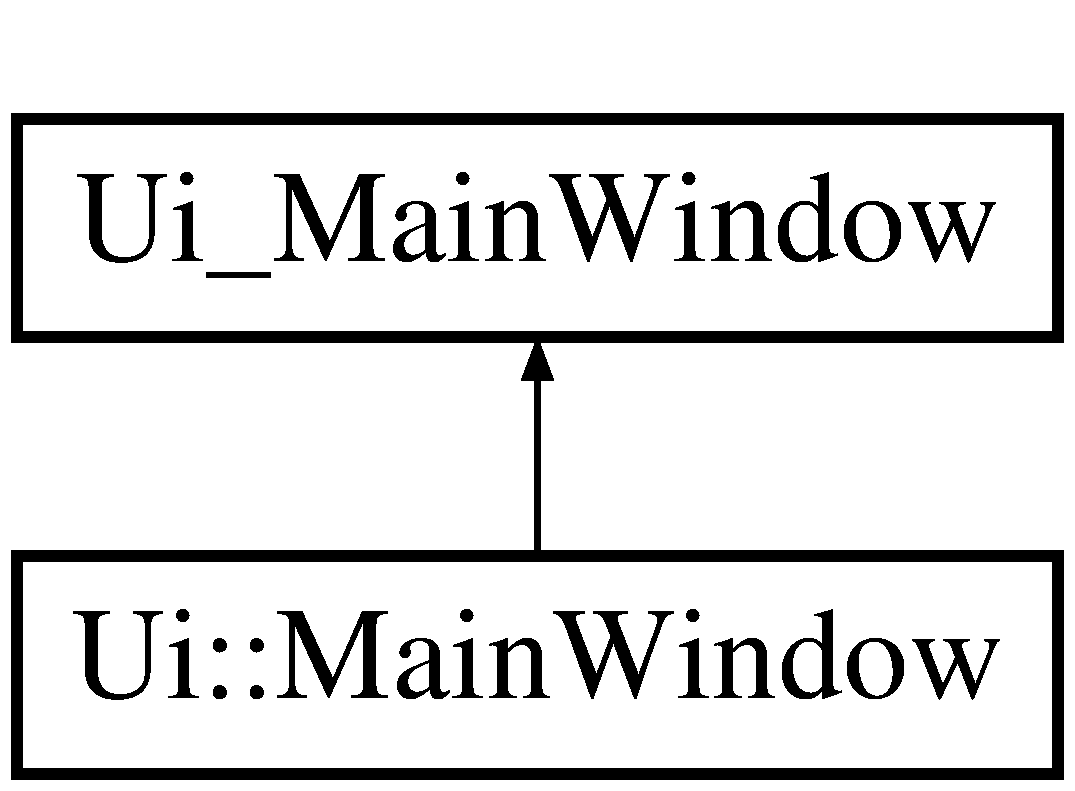
\includegraphics[height=2.000000cm]{class_ui___main_window}
\end{center}
\end{figure}
\subsection*{Public Member Functions}
\begin{DoxyCompactItemize}
\item 
\mbox{\Hypertarget{class_ui___main_window_acf4a0872c4c77d8f43a2ec66ed849b58}\label{class_ui___main_window_acf4a0872c4c77d8f43a2ec66ed849b58}} 
void {\bfseries setup\+Ui} (Q\+Main\+Window $\ast$Main\+Window)
\item 
\mbox{\Hypertarget{class_ui___main_window_a097dd160c3534a204904cb374412c618}\label{class_ui___main_window_a097dd160c3534a204904cb374412c618}} 
void {\bfseries retranslate\+Ui} (Q\+Main\+Window $\ast$Main\+Window)
\end{DoxyCompactItemize}
\subsection*{Public Attributes}
\begin{DoxyCompactItemize}
\item 
\mbox{\Hypertarget{class_ui___main_window_a356f1cf3ebda15f1fac59467ee081b74}\label{class_ui___main_window_a356f1cf3ebda15f1fac59467ee081b74}} 
Q\+Widget $\ast$ {\bfseries centralwidget}
\item 
\mbox{\Hypertarget{class_ui___main_window_adf43d9a67adaec750aaa956b5e082f09}\label{class_ui___main_window_adf43d9a67adaec750aaa956b5e082f09}} 
Q\+Menu\+Bar $\ast$ {\bfseries menubar}
\item 
\mbox{\Hypertarget{class_ui___main_window_a1687cceb1e2787aa1f83e50433943a91}\label{class_ui___main_window_a1687cceb1e2787aa1f83e50433943a91}} 
Q\+Status\+Bar $\ast$ {\bfseries statusbar}
\end{DoxyCompactItemize}


The documentation for this class was generated from the following file\+:\begin{DoxyCompactItemize}
\item 
client\+\_\+interface/interface\+\_\+autogen/include/ui\+\_\+mainwindow.\+h\end{DoxyCompactItemize}

%--- End generated contents ---

% Index
\backmatter
\newpage
\phantomsection
\clearemptydoublepage
\addcontentsline{toc}{chapter}{Index}
\printindex

\end{document}
